\documentclass[aspectratio=169]{beamer}
% ============================================================================
% HEC Montréal MBA -- ECON50803: Macroeconomic Environment
% Shared Beamer Preamble
% ============================================================================

% --- Theme and base settings ------------------------------------------------
\usetheme{default}
\setbeamersize{text margin left=1.2cm, text margin right=1.2cm}

% --- Fonts ------------------------------------------------------------------
% Sans-serif throughout for a business look (comment out FiraSans if unavailable)
\usepackage[sfdefault,light]{FiraSans}
\usepackage{FiraMono}
\usepackage[T1]{fontenc}
\usepackage[utf8]{inputenc}
\setbeamerfont{title}{series=\bfseries, size=\Large}
\setbeamerfont{frametitle}{series=\bfseries, size=\large}
\setbeamerfont{framesubtitle}{series=\mdseries, size=\normalsize}

% --- Colors -----------------------------------------------------------------
\definecolor{HECnavy}{HTML}{002855}
\definecolor{HECgreen}{HTML}{26d07c}
\definecolor{HECcoral}{HTML}{ff585d}
\definecolor{HECtext}{HTML}{2D3748}
\definecolor{HECgray}{HTML}{94A3B8}
\definecolor{HEClightgray}{HTML}{F1F5F9}
\definecolor{HEClightblue}{HTML}{E8EDF3}

% Beamer color assignments
\setbeamercolor{normal text}{fg=HECtext}
\setbeamercolor{title}{fg=HECnavy}
\setbeamercolor{frametitle}{fg=HECnavy}
\setbeamercolor{structure}{fg=HECnavy}
\setbeamercolor{background canvas}{bg=white}
\setbeamercolor{alerted text}{fg=HECcoral}
\setbeamercolor{example text}{fg=HECgreen}
\hypersetup{colorlinks, linkcolor=HECnavy, urlcolor=HECnavy, citecolor=HECtext}

% --- Navigation and chrome --------------------------------------------------
\setbeamertemplate{navigation symbols}{}

% Frame title: bold text with a thin accent line
\setbeamertemplate{frametitle}{%
   \vspace{0.25cm}%
   {\usebeamerfont{frametitle}\usebeamercolor[fg]{frametitle}\insertframetitle}%
   \ifx\insertframesubtitle\empty\else%
      \\[2pt]{\usebeamerfont{framesubtitle}\textcolor{HECgray}{\insertframesubtitle}}%
   \fi%
   \\[-4pt]\textcolor{HECgreen}{\rule{2.5cm}{1.5pt}}%
   \\[-2pt]%
}

% Footer: course name left, slide number right, thin rule above
\setbeamertemplate{footline}{%
   \vspace{-0.1cm}%
   \hbox to \paperwidth{%
      \hspace{1.2cm}%
      \textcolor{HEClightgray}{\rule{0.84\paperwidth}{0.4pt}}%
      \hspace{1.2cm}%
   }%
   \vspace{0.05cm}%
   \hbox to \paperwidth{%
      \hspace{1.2cm}%
      {\scriptsize\textcolor{HECgray}{ECON 50803\enspace\textbar\enspace Environnement macroéconomique}}%
      \hfill%
      {\scriptsize\textcolor{HECgray}{\insertframenumber}}%
      \hspace{1.2cm}%
   }%
   \vspace{0.15cm}%
}

% --- Itemize/enumerate styling ----------------------------------------------
\setbeamertemplate{itemize item}{\textcolor{HECnavy}{$\bullet$}}
\setbeamertemplate{itemize subitem}{\textcolor{HECgray}{$\bullet$}}
\setbeamertemplate{itemize subsubitem}{\textcolor{HECgray}{\scalebox{0.6}{$\blacktriangleright$}}}
\setbeamertemplate{enumerate item}{\textcolor{HECnavy}{\bfseries\insertenumlabel.}}
\setbeamertemplate{enumerate subitem}{\textcolor{HECgray}{\insertsubenumlabel.}}

% --- Packages ---------------------------------------------------------------
\usepackage{
   tikz, caption, subcaption, ragged2e, amsmath, bm,
   makecell, threeparttable, booktabs, mathtools,
   multirow, calc, hyperref, tabularx, colortbl,
   transparent, tcolorbox, xcolor, graphicx
}
\usepackage[round]{natbib}
\usetikzlibrary{decorations.pathreplacing, decorations.markings, calc, arrows.meta, positioning}
\usepackage[absolute,overlay]{textpos}
\captionsetup[figure]{labelformat=empty, font=small, textfont=it}
\captionsetup[table]{labelformat=empty, font=small}
\setlength{\belowcaptionskip}{0cm}
\apptocmd{\frame}{}{\justifying}

% --- Paths ------------------------------------------------------------------
\graphicspath{{../Figures/}}
\newcommand*\includetables[1]{\input{../Tables/#1.tex}}

% --- Mathematical commands --------------------------------------------------
\DeclareMathOperator*{\argmax}{arg\,max}
\newcommand{\partialof}[2]{\frac{\partial #1}{\partial #2}}
\newcommand{\totalof}[2]{\frac{\text{d}#1}{\text{d}#2}}
\newcommand{\pctchg}[1]{\%\Delta #1}
\newcommand{\smallquad}{\hspace{0.5em}}

% --- Resize equation command ------------------------------------------------
\newcommand{\resizeeq}[2]{\resizebox{#2\hsize}{!}{$#1$}}

% ============================================================================
% CUSTOM SLIDE TYPES
% ============================================================================

% --- Title slide (call with \titleframe) ------------------------------------
\newcommand{\titleframe}{%
   {\setbeamertemplate{footline}{}%
   \begin{frame}[plain]
      \begin{tikzpicture}[remember picture, overlay]
         % Navy accent bar on the left
         \fill[HECnavy] (current page.north west) rectangle
            ([xshift=0.6cm]current page.south west);
         % Green accent line
         \fill[HECgreen] ([xshift=0.6cm]current page.north west) rectangle
            ([xshift=0.65cm]current page.south west);
      \end{tikzpicture}
      \vspace{1cm}
      \hspace{0.6cm}%
      \begin{minipage}{0.85\textwidth}
         {\usebeamerfont{title}\usebeamercolor[fg]{title}\inserttitle}
         \\[12pt]
         \textcolor{HECgreen}{\rule{3cm}{2pt}}
         \\[12pt]
         {\large\textcolor{HECgray}{\insertauthor}}
         \\[6pt]
         {\normalsize\textcolor{HECgray}{\insertdate}}
      \end{minipage}
      \vfill
      \hspace{0.6cm}%
      {\footnotesize\textcolor{HECgray}{HEC Montréal \enspace\textbar\enspace MBA}}
      \vspace{0.5cm}
   \end{frame}}%
}

% --- Section divider slide --------------------------------------------------
\newcommand{\sectionframe}[1]{%
   {\setbeamertemplate{footline}{}%
   \begin{frame}[plain]
      \begin{tikzpicture}[remember picture, overlay]
         \fill[HECnavy] ([shift={(-1pt,1pt)}]current page.north west) rectangle
            ([shift={(1pt,-1pt)}]current page.south east);
         \node[anchor=center] at (current page.center) {%
            \begin{minipage}{0.8\paperwidth}
               \centering
               {\LARGE\bfseries\textcolor{white}{#1}}
               \\[12pt]
               \textcolor{HECgreen}{\rule{3cm}{2pt}}
            \end{minipage}
         };
      \end{tikzpicture}
   \end{frame}}%
}

% ============================================================================
% CUSTOM BOX ENVIRONMENTS
% ============================================================================

% Key Insight (green accent)
\newtcolorbox{keyinsight}[1][Point clé]{%
   colback=HECgreen!5,
   colframe=HECgreen,
   boxrule=0pt,
   leftrule=3pt,
   arc=8pt,
   title={\textcolor{HECgreen}{\bfseries #1}},
   coltitle=HECgreen,
   fonttitle=\bfseries,
   attach title to upper={\\[4pt]},
   left=10pt, right=10pt, top=6pt, bottom=6pt
}

% Business Implication (navy accent)
\newtcolorbox{bizimplication}[1][Implication d'affaires]{%
   colback=HECnavy!5,
   colframe=HECnavy,
   boxrule=0pt,
   leftrule=3pt,
   arc=8pt,
   title={\textcolor{HECnavy}{\bfseries #1}},
   coltitle=HECnavy,
   fonttitle=\bfseries,
   attach title to upper={\\[4pt]},
   left=10pt, right=10pt, top=6pt, bottom=6pt
}

% Warning / Important (coral accent)
\newtcolorbox{warning}[1][Important]{%
   colback=HECcoral!5,
   colframe=HECcoral,
   boxrule=0pt,
   leftrule=3pt,
   arc=8pt,
   title={\textcolor{HECcoral}{\bfseries #1}},
   coltitle=HECcoral,
   fonttitle=\bfseries,
   attach title to upper={\\[4pt]},
   left=10pt, right=10pt, top=6pt, bottom=6pt
}

% Definition (gray background)
\newtcolorbox{defbox}[1][Définition]{%
   colback=HEClightgray,
   colframe=HEClightgray,
   boxrule=0pt,
   leftrule=3pt,
   arc=8pt,
   left=10pt, right=10pt, top=6pt, bottom=6pt,
   title={\textcolor{HECnavy}{\bfseries #1}},
   coltitle=HECnavy,
   fonttitle=\bfseries,
   attach title to upper={\\[4pt]}
}

% In-Class Exercise (coral accent)
\newtcolorbox{exercise}[1][Exercice]{%
   colback=HECcoral!5,
   colframe=HECcoral,
   boxrule=0pt,
   leftrule=3pt,
   arc=8pt,
   title={\textcolor{HECcoral}{\bfseries #1}},
   coltitle=HECcoral,
   fonttitle=\bfseries,
   attach title to upper={\\[4pt]},
   left=10pt, right=10pt, top=6pt, bottom=6pt
}

% ============================================================================
% NEWSPAPER HEADLINES SLIDE TEMPLATE
% ============================================================================
% Usage: inside a frame, open a tikzpicture[remember picture, overlay], then:
%   \setcounter{newshl}{0}
%   \newsheadline{Newspaper Name}{``Headline text''}   % up to 6 entries
%   \headlinesoverlay{Large overlay text}               % optional 2nd slide
%
% Headlines are auto-positioned in a 2×3 staggered grid (left/right alternating).
%
% Logo support: place PNG files in Figures/logos/ (e.g., ft.png, economist.png).
% Use the optional argument to specify the logo file (without extension):
%   \newsheadline[ft]{Financial Times}{Headline text}   % logo + bold headline
%   \newsheadline{The Economist}{``Headline text''}      % text-only fallback

\newcounter{newshl}

\newcommand{\newsheadline}[3][]{%
   % #1 = optional logo file key (e.g., ft → logos/ft.png)
   % #2 = newspaper name (text fallback when no logo)
   % #3 = headline text
   \stepcounter{newshl}%
   \pgfmathsetmacro{\hlrow}{int((\thenewshl-1)/2)}%
   \pgfmathsetmacro{\hlcol}{int(mod(\thenewshl-1,2))}%
   \pgfmathsetmacro{\hlx}{0.8 + \hlcol * 7.8}%
   \pgfmathsetmacro{\hly}{-1.5 - \hlrow * 2.0}%
   \node[anchor=north west]
      at ([shift={(\hlx cm,\hly cm)}]current page.north west) {%
      \ifx\\#1\\%
         \begin{minipage}[t]{5.8cm}%
            \textbf{\textcolor{HECgray}{\footnotesize\MakeUppercase{#2}}}%
            \\[-1pt]%
            {\small\itshape #3}%
         \end{minipage}%
      \else%
         \begin{minipage}[c]{1.2cm}%
            \includegraphics[height=1.2cm]{logos/#1}%
         \end{minipage}%
         \hspace{6pt}%
         \begin{minipage}[c][1.2cm][c]{4.3cm}%
            \raggedright{\small\textcolor{HECtext!75}{#3}}%
         \end{minipage}%
      \fi%
   };%
}

\newcommand{\headlinesoverlay}[1]{%
   \only<2>{%
      \fill[white, opacity=0.85]
         (current page.south west) rectangle (current page.north east);%
      \node[anchor=center] at ([yshift=-0.5cm]current page.center) {%
         {\fontsize{36}{44}\selectfont\bfseries\textcolor{HECnavy}{#1}}%
      };%
   }%
}

% ============================================================================
% NAVIGATION BUTTONS (optional, for bottom-of-slide section nav)
% ============================================================================

\newlength{\buttonwidth}
\newlength{\currentxpos}
\setlength{\currentxpos}{1.2cm}
\newlength{\buttonsep}
\setlength{\buttonsep}{0.05cm}

\newcommand{\mybutton}[2]{%
   \settowidth{\buttonwidth}{#1}%
   \begin{textblock*}{\buttonwidth + 2ex}(\currentxpos, \paperheight - 2.5em)
      \hyperlink{#2}{\beamerbutton{#1}}
   \end{textblock*}%
   \addtolength{\currentxpos}{\buttonwidth + \buttonsep}%
}

% ============================================================================
% BACKUP SLIDES SUPPORT
% ============================================================================

\newcommand{\backupbegin}{%
   \newcounter{finalframe}%
   \setcounter{finalframe}{\value{framenumber}}%
}
\newcommand{\backupend}{%
   \setcounter{framenumber}{\value{finalframe}}%
}


\title{Politique mon\'{e}taire et budg\'{e}taire}
\author{Jean-F\'elix Brouillette}
\date{S\'eance 5}

\begin{document}

% ============================================================================
\titleframe
% ============================================================================

% --- Opening hook: newspaper headlines ---
{
\setbeamertemplate{footline}{}
\begin{frame}{Les d\'{e}cideurs face \`{a} la temp\^{e}te}
   \begin{tikzpicture}[remember picture, overlay]
      \setcounter{newshl}{0}
      \newsheadline[lapresse]{La Presse}{\guillemotleft~La Banque du Canada abaisse son taux directeur pour la sixi\`{e}me fois cons\'{e}cutive~\guillemotright}
      \newsheadline[ft]{Financial Times}{\guillemotleft~Central banks grapple with Trump tariffs as inflation risks rise~\guillemotright}
      \newsheadline[globeandmail]{The Globe and Mail}{\guillemotleft~Ottawa signals new spending to shore up economy amid trade war~\guillemotright}
      \newsheadline[bloomberg]{Bloomberg}{\guillemotleft~ECB cuts rates to 2.75\% as euro-area growth stalls~\guillemotright}
      \newsheadline[radiocanada]{Radio-Canada}{\guillemotleft~Faut-il s'inqui\'{e}ter de la dette publique canadienne\,?~\guillemotright}
      \newsheadline[economist]{The Economist}{\guillemotleft~The case for more fiscal firepower~\guillemotright}
   \end{tikzpicture}
\end{frame}
}

\begin{frame}{Un instrument puissant\ldots}
   \begin{figure}
      \centering
      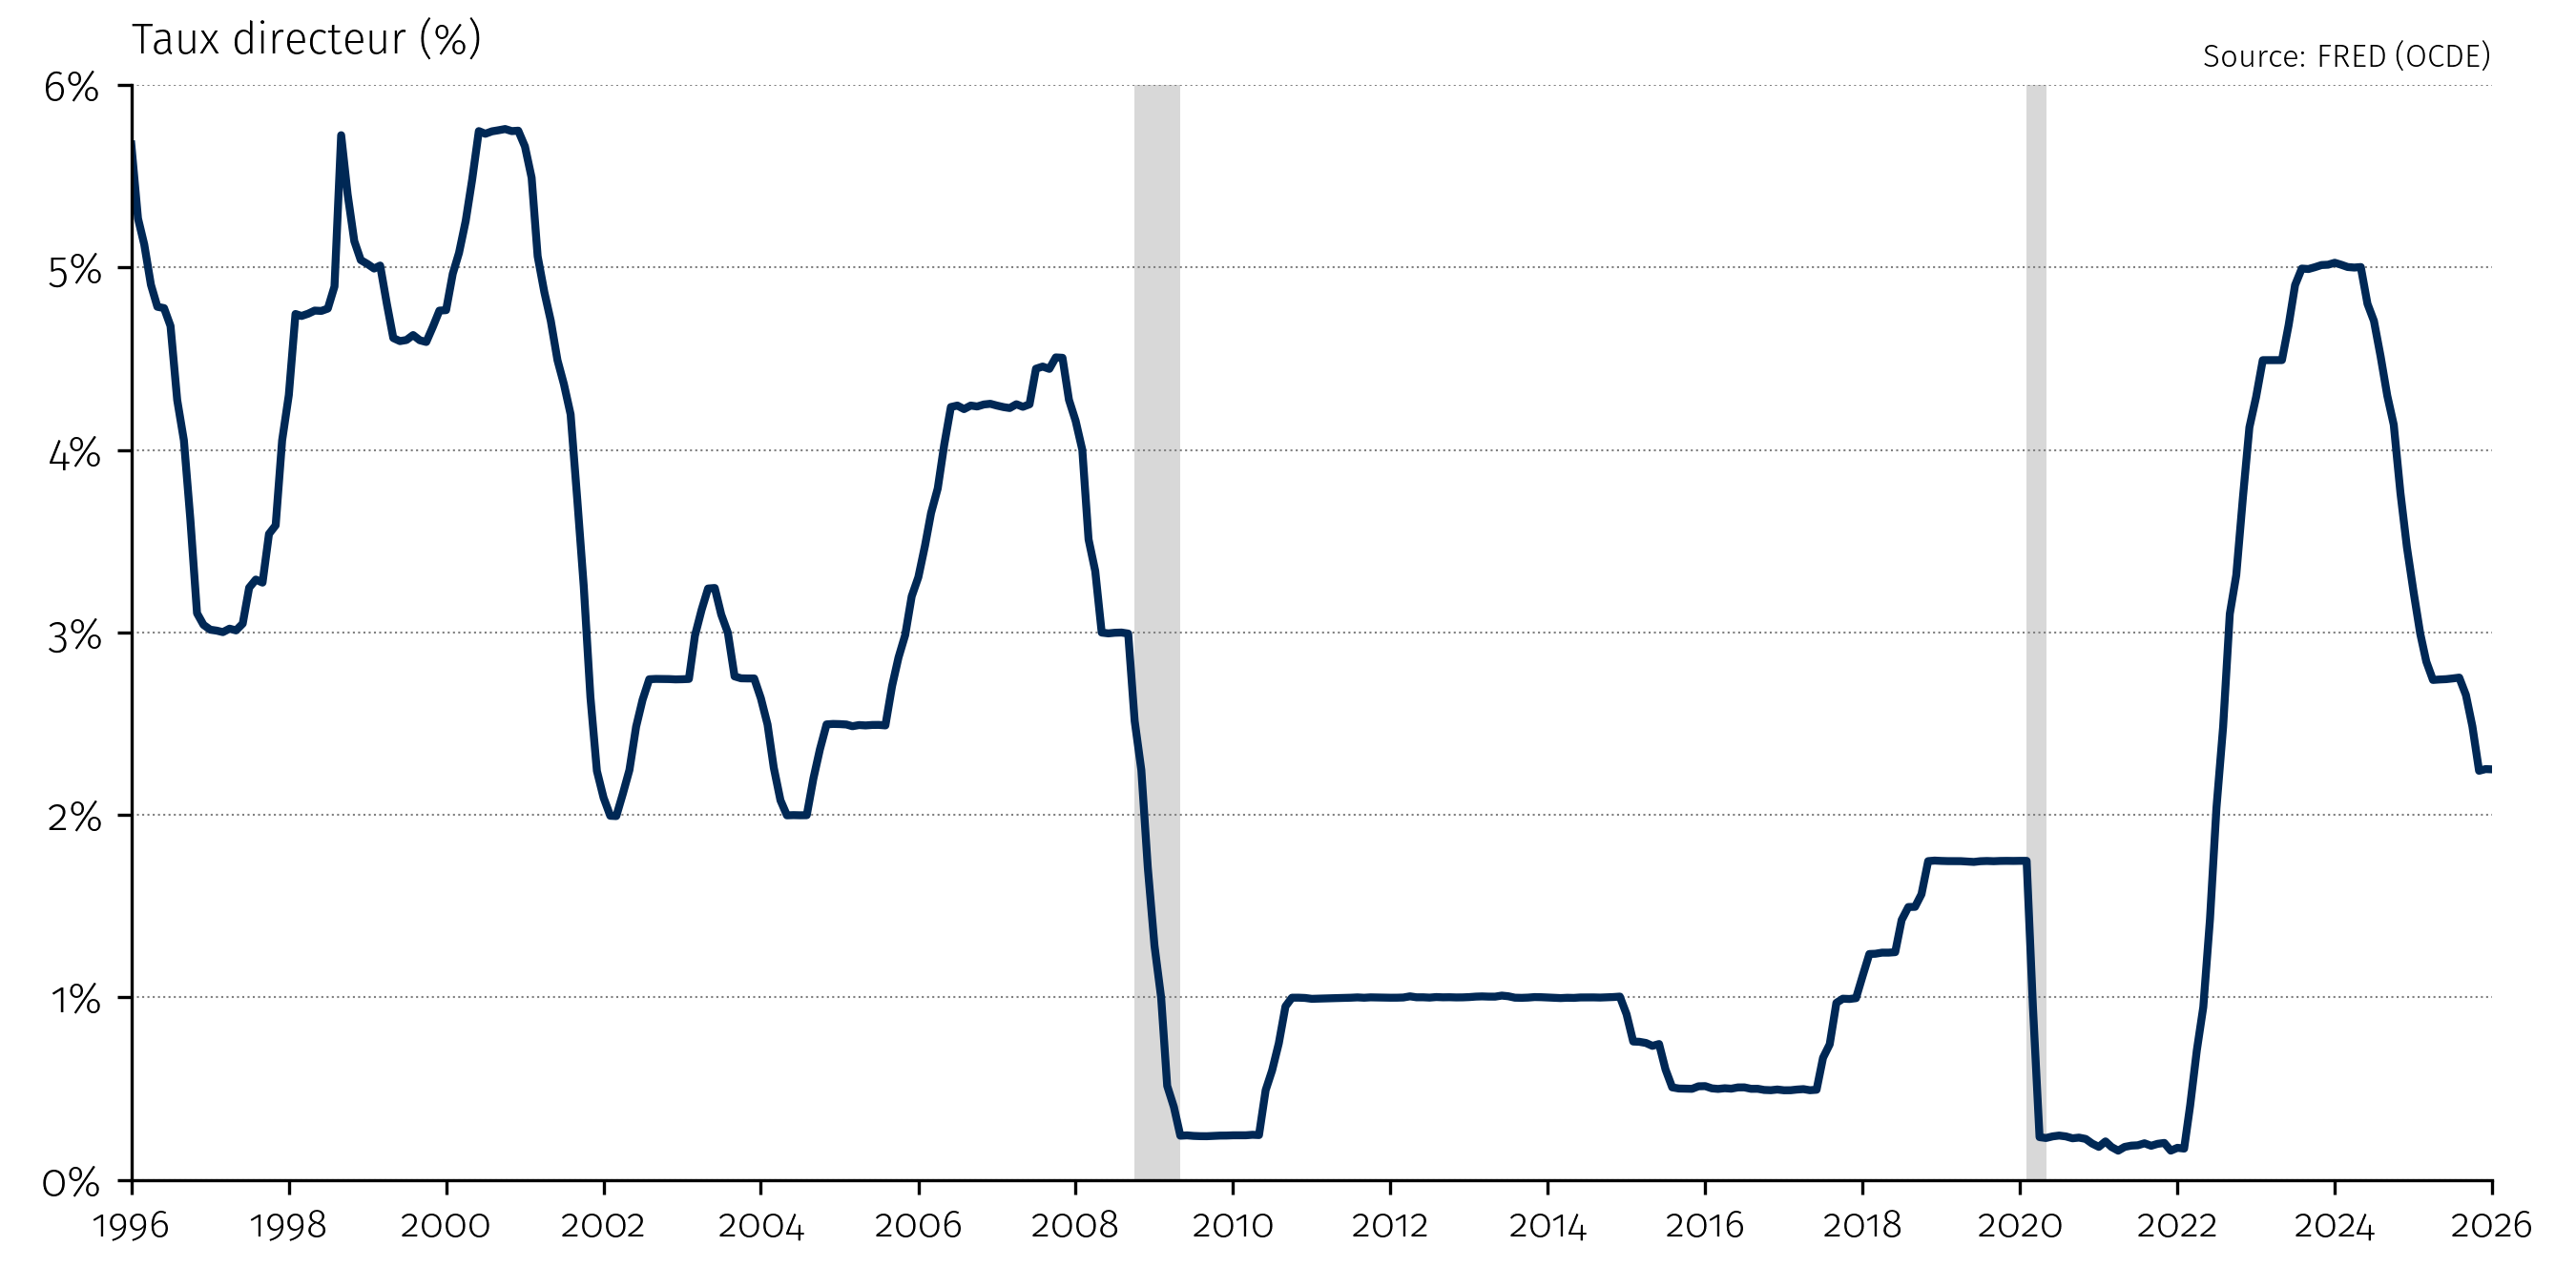
\includegraphics[width=0.95\textwidth, height=0.78\textheight, keepaspectratio]{overnight_rate_ca.png}
   \end{figure}
\end{frame}

\begin{frame}{\ldots qui touche tout le monde}
   \begin{figure}
      \centering
      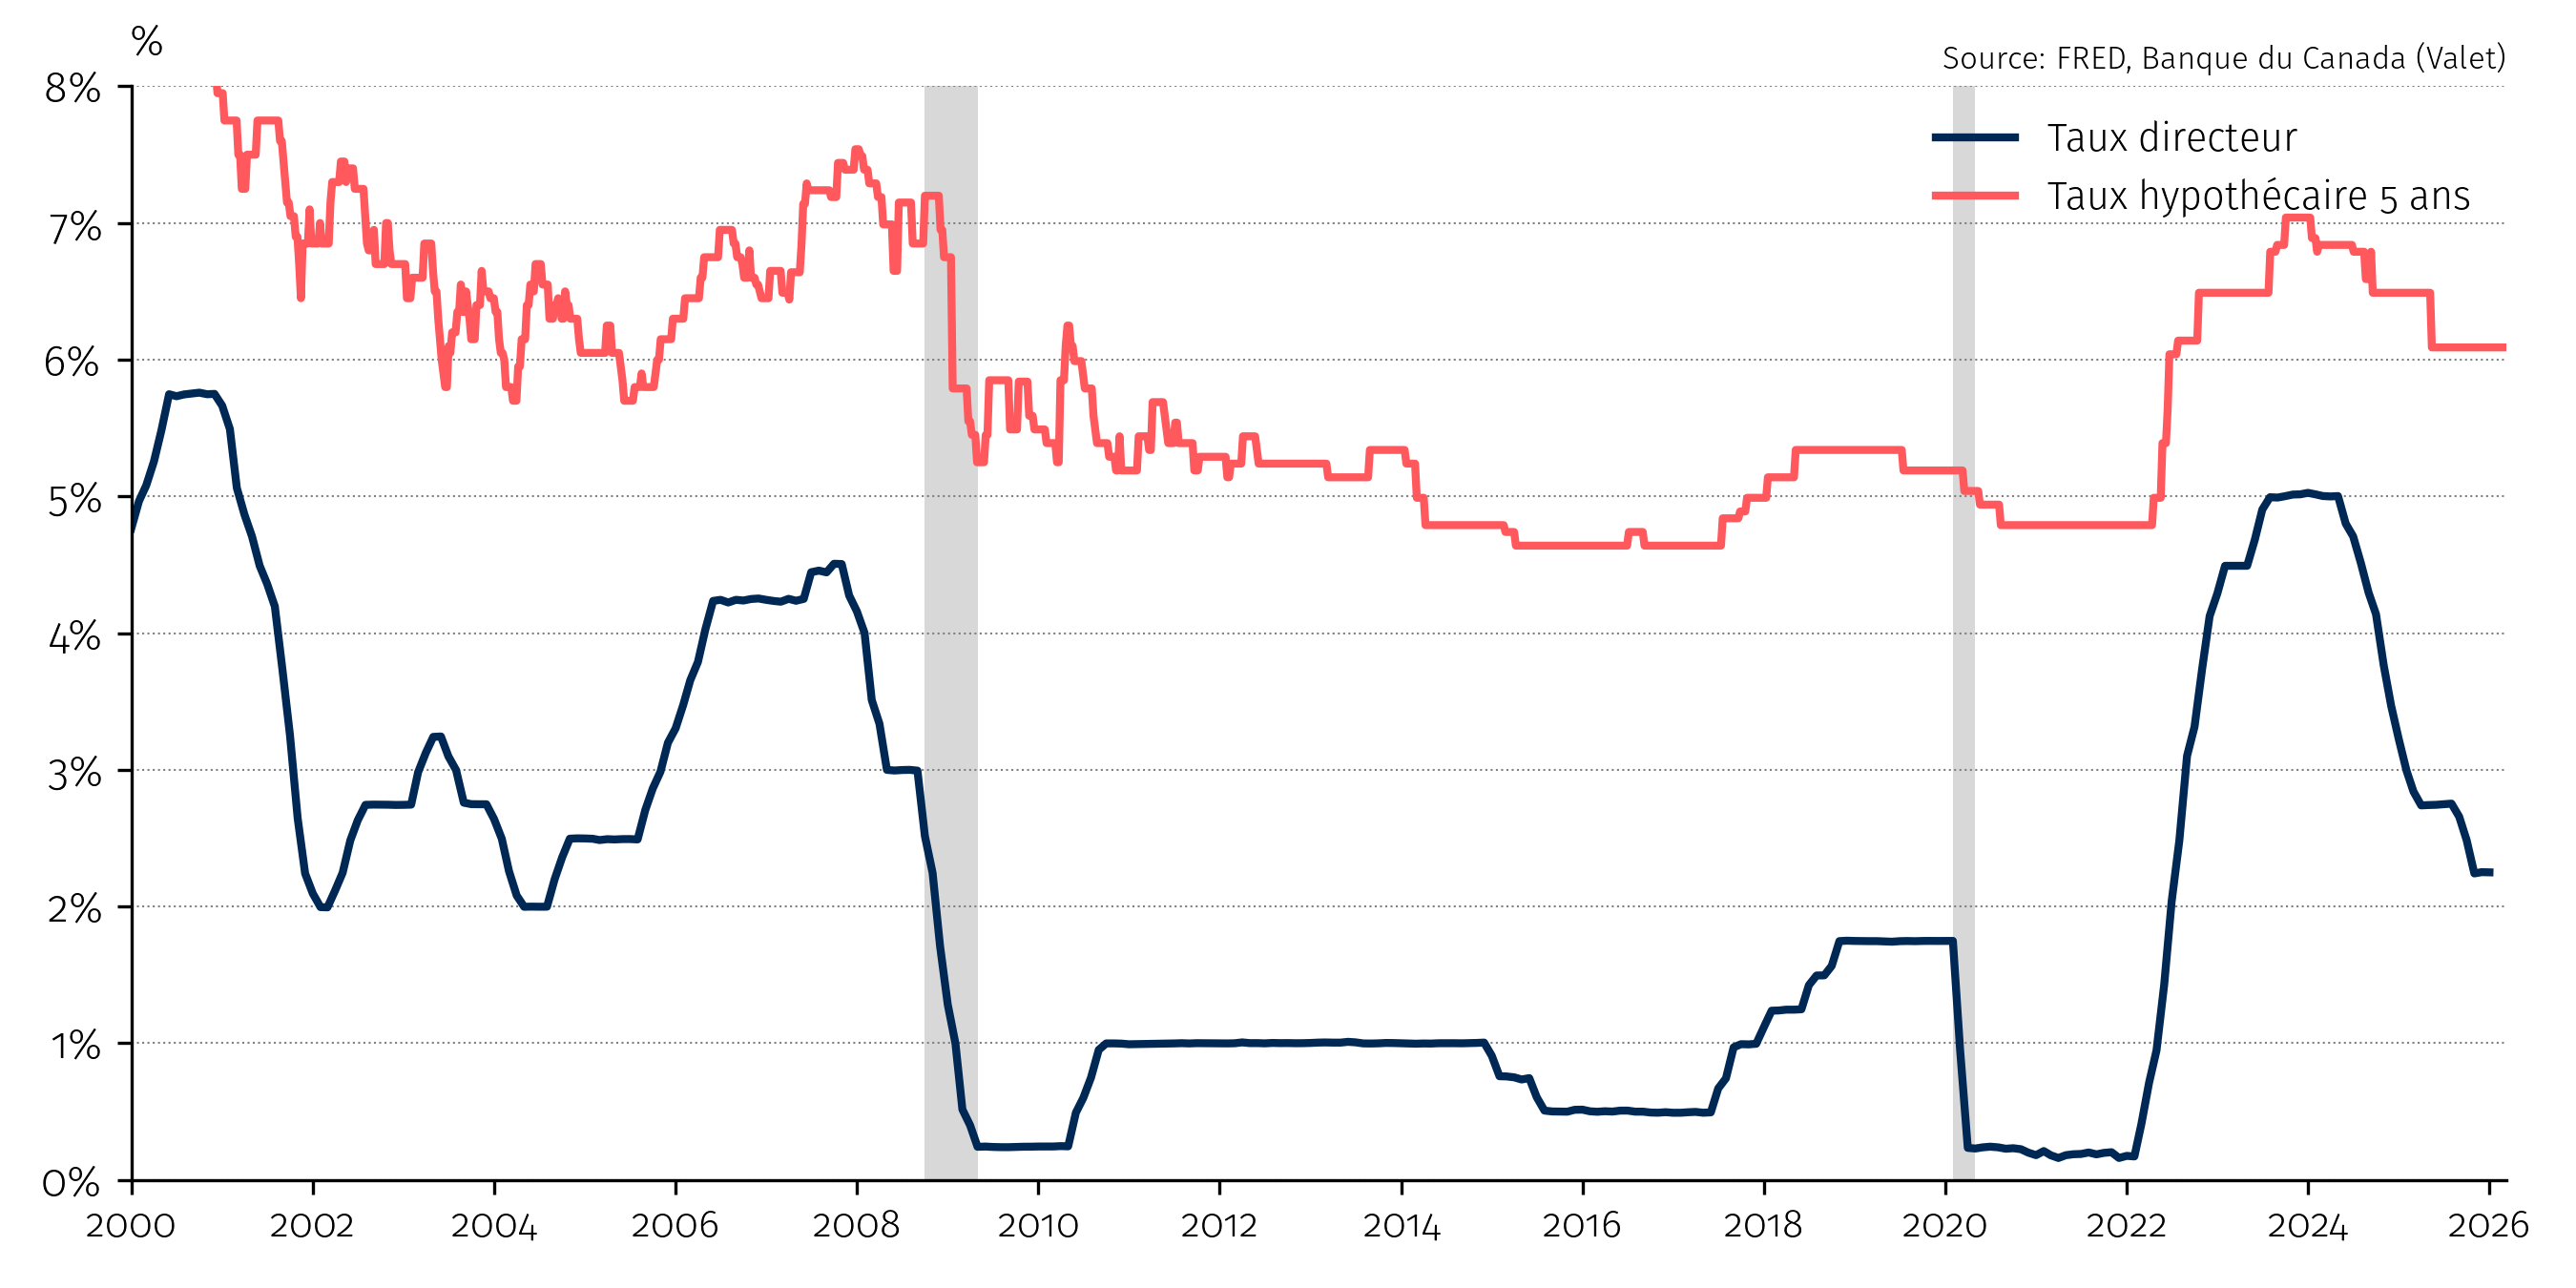
\includegraphics[width=0.95\textwidth, height=0.78\textheight, keepaspectratio]{overnight_vs_mortgage.png}
   \end{figure}
\end{frame}

% ============================================================================
% PLAN
% ============================================================================

\begin{frame}{Plan}
   \begin{enumerate}
      \setlength\itemsep{0.5cm}
      \item \textbf{Pourquoi combattre les r\'{e}cessions\,?}
      \item La politique mon\'{e}taire conventionnelle
      \item D\'{e}fis et limites de la politique mon\'{e}taire
      \item La politique mon\'{e}taire non conventionnelle
      \item La politique budg\'{e}taire
      \item La dette publique
   \end{enumerate}
\end{frame}

% ============================================================================
\sectionframe{Pourquoi combattre les r\'{e}cessions\,?}
% ============================================================================

\begin{frame}[t]{Pourquoi ne pas laissez les prix faire leur boulot\,?}
   \small
   \begin{columns}[T]
      \begin{column}{0.45\textwidth}
         \textbf{\textcolor{HECnavy}{R\'{e}cession} ($Y < Y_{\text{POT}}$)}
         \vspace{0.1cm}
         \begin{enumerate}
            \setlength\itemsep{0.08cm}
            \item Ch\^{o}mage \'{e}lev\'{e}
            \item Travailleurs abondants
            \item Baisse des salaires nominaux
            \item Baisse des co\^{u}ts de production
            \item Hausse des profits et de l'offre
            \item[\textcolor{HECnavy}{$\to$}] \textbf{AS se d\'{e}place vers la droite}
         \end{enumerate}
      \end{column}
      \begin{column}{0.45\textwidth}
         \textbf{\textcolor{HECcoral}{Surchauffe} ($Y > Y_{\text{POT}}$)}
         \vspace{0.1cm}
         \begin{enumerate}
            \setlength\itemsep{0.08cm}
            \item Chômage faible
            \item Travailleurs rares
            \item Hausse des salaires nominaux
            \item Hausse des co\^{u}ts de production
            \item Baisse des profits et de l'offre
            \item[\textcolor{HECcoral}{$\to$}] \textbf{AS se d\'{e}place vers la gauche}
         \end{enumerate}
      \end{column}
   \end{columns}
   \vspace{0.15cm}
   \begin{keyinsight}
      Après un certain temps, les salaires et coûts de production \textbf{s'ajustent naturellement} et l'\'{e}conomie revient vers $Y_{\text{POT}}$. Alors pourquoi combattre les r\'{e}cessions\,?
   \end{keyinsight}
\end{frame}

\begin{frame}[t]{Choc de demande n\'{e}gatif : le choc}
   \vspace{0.1cm}
   \begin{columns}[T]
      \begin{column}{0.55\textwidth}
         \centering
         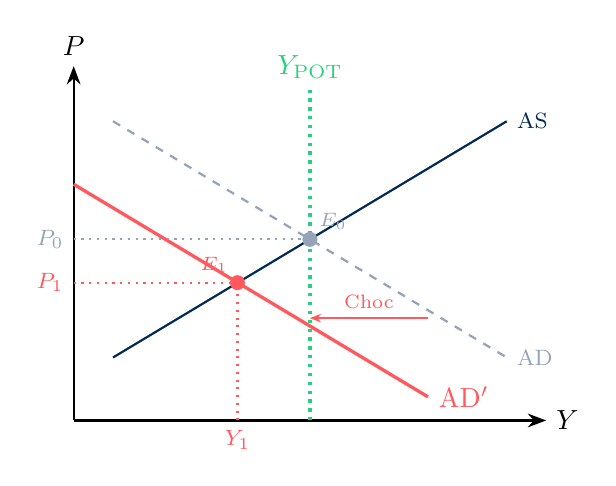
\begin{tikzpicture}[scale=1.0]
            % Axes
            \draw[-{Stealth}, thick] (0,0) -- (6,0) node[right] {$Y$};
            \draw[-{Stealth}, thick] (0,0) -- (0,4.5) node[above] {$P$};
            % Y_POT
            \draw[HECgreen, very thick, dotted] (3.0,0) -- (3.0,4.2)
               node[above] {$Y_{\text{POT}}$};
            % AS: y = 0.6x + 0.5
            \draw[HECnavy, thick] (0.5,0.8) -- (5.5,3.8)
               node[right, font=\footnotesize] {AS};
            % AD original (dashed): y = -0.6x + 4.1
            \draw[HECgray, dashed, thick] (0.5,3.8) -- (5.5,0.8)
               node[right, font=\footnotesize] {AD};
            % AD' shifted left: y = -0.6x + 3.0
            \draw[HECcoral, very thick] (0.0,3.0) -- (4.5,0.3)
               node[right] {AD$'$};
            % E0: AD ∩ AS at (3.0, 2.3)
            \filldraw[HECgray] (3.0,2.3) circle (2.5pt);
            \node[font=\scriptsize, HECgray, above right] at (3.0,2.3) {$E_0$};
            % E1: AD' ∩ AS at (2.08, 1.75)
            \filldraw[HECcoral] (2.08,1.75) circle (2.5pt);
            \node[font=\scriptsize, HECcoral, above left] at (2.08,1.75) {$E_1$};
            % Shock arrow (AD → AD') at y=1.3: AD at x=4.67, AD' at x=2.83
            \draw[-{Stealth[length=4pt]}, HECcoral, thick] (4.5,1.3) -- (3.0,1.3);
            \node[font=\scriptsize, HECcoral, above] at (3.75,1.3) {Choc};
            % Dotted reference lines
            \draw[dotted, thick, HECcoral] (2.08,0) node[below, font=\footnotesize] {$Y_1$} -- (2.08,1.75);
            \draw[dotted, thick, HECgray] (0,2.3) node[left, font=\footnotesize] {$P_0$} -- (3.0,2.3);
            \draw[dotted, thick, HECcoral] (0,1.75) node[left, font=\footnotesize] {$P_1$} -- (2.08,1.75);
         \end{tikzpicture}
      \end{column}
      \begin{column}{0.42\textwidth}
         \small
         \textbf{Court terme :}
         \vspace{0.15cm}
         \begin{enumerate}
            \setlength\itemsep{0.15cm}
            \item AD se d\'{e}place \`{a} gauche
            \item Nouvel \'{e}quilibre $E_1$ : $Y$ $\downarrow$ $+$ $P$ $\downarrow$
            \item $Y_1 < Y_{\text{POT}}$ $\to$ r\'{e}cession
         \end{enumerate}
         \vspace{0.3cm}
         \textcolor{HECgray}{\footnotesize L'\'{e}conomie est en dessous de son potentiel. Que se passe-t-il ensuite\,?}
      \end{column}
   \end{columns}
\end{frame}

\begin{frame}[t]{Choc de demande n\'{e}gatif : l'ajustement naturel}
   \vspace{0.1cm}
   \begin{columns}[T]
      \begin{column}{0.55\textwidth}
         \centering
         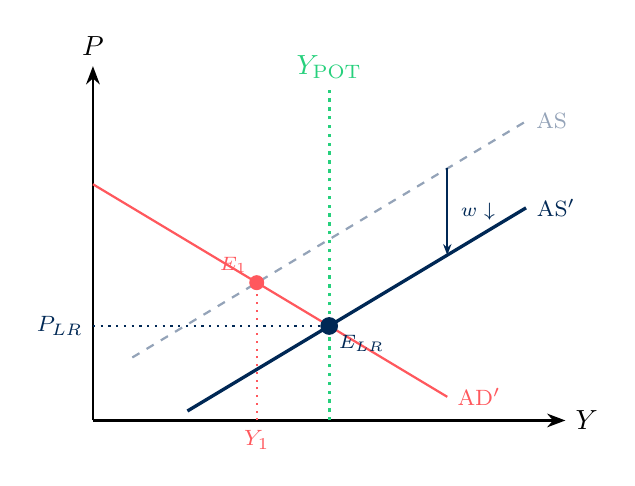
\begin{tikzpicture}[scale=1.0]
            % Axes
            \draw[-{Stealth}, thick] (0,0) -- (6,0) node[right] {$Y$};
            \draw[-{Stealth}, thick] (0,0) -- (0,4.5) node[above] {$P$};
            % Y_POT
            \draw[HECgreen, very thick, dotted] (3.0,0) -- (3.0,4.2)
               node[above] {$Y_{\text{POT}}$};
            % AS original (dashed): y = 0.6x + 0.5
            \draw[HECgray, dashed, thick] (0.5,0.8) -- (5.5,3.8)
               node[right, font=\footnotesize] {AS};
            % AD' (solid, the new demand): y = -0.6x + 3.0
            \draw[HECcoral, thick] (0.0,3.0) -- (4.5,0.3)
               node[right, font=\footnotesize] {AD$'$};
            % AS' shifted right: y = 0.6x - 0.6 (passes through Y_POT at P=1.2)
            \draw[HECnavy, very thick] (1.2,0.12) -- (5.5,2.7)
               node[right, font=\footnotesize] {AS$'$};
            % E1: AD' ∩ AS at (2.08, 1.75)
            \filldraw[HECcoral] (2.08,1.75) circle (2.5pt);
            \node[font=\scriptsize, HECcoral, above left] at (2.08,1.75) {$E_1$};
            % E_LR: AD' ∩ AS' at (3.0, 1.2)
            \filldraw[HECnavy] (3.0,1.2) circle (3pt);
            \node[font=\scriptsize, HECnavy, below right] at (3.0,1.2) {$E_{LR}$};
            % AS adjustment arrow (AS → AS') at x=4.5: AS at y=3.2, AS' at y=2.1
            \draw[-{Stealth[length=4pt]}, HECnavy, thick] (4.5,3.2) -- (4.5,2.1);
            \node[font=\scriptsize, HECnavy, right] at (4.55,2.65) {$w\downarrow$};
            % Dotted reference lines
            \draw[dotted, thick, HECcoral] (2.08,0) node[below, font=\footnotesize] {$Y_1$} -- (2.08,1.75);
            \draw[dotted, thick, HECnavy] (0,1.2) node[left, font=\footnotesize] {$P_{LR}$} -- (3.0,1.2);
         \end{tikzpicture}
      \end{column}
      \begin{column}{0.42\textwidth}
         \small
         \textbf{Long terme :}
         \vspace{0.15cm}
         \begin{enumerate}
            \setlength\itemsep{0.1cm}
            \item $Y_1 < Y_{\text{POT}}$ $\to$ ch\^{o}mage \'{e}lev\'{e}
            \item Travailleurs abondants
            \item Salaires nominaux $\downarrow$ $\to$ co\^{u}ts $\downarrow$
            \item AS se d\'{e}place vers la droite
            \item Retour \`{a} $Y_{\text{POT}}$ au prix $P_{LR}$
         \end{enumerate}
         \vspace{0.2cm}
         \textcolor{HECgray}{\footnotesize M\^{e}me niveau de production, mais à un niveau de prix plus bas.}
      \end{column}
   \end{columns}
\end{frame}

\begin{frame}[t]{Choc de demande positif : le choc}
   \vspace{0.1cm}
   \begin{columns}[T]
      \begin{column}{0.55\textwidth}
         \centering
         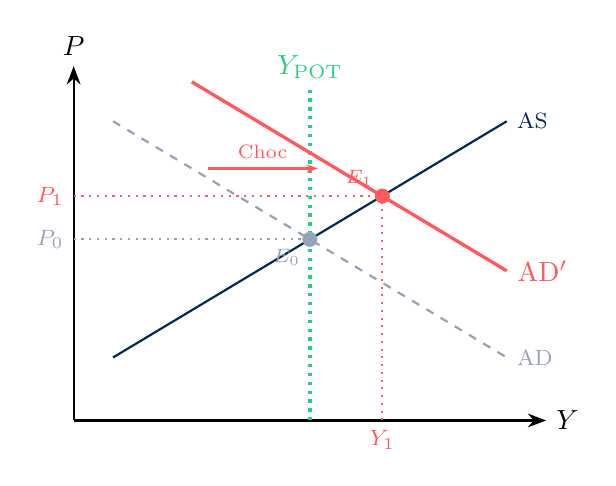
\begin{tikzpicture}[scale=1.0]
            % Axes
            \draw[-{Stealth}, thick] (0,0) -- (6,0) node[right] {$Y$};
            \draw[-{Stealth}, thick] (0,0) -- (0,4.5) node[above] {$P$};
            % Y_POT
            \draw[HECgreen, very thick, dotted] (3.0,0) -- (3.0,4.2)
               node[above] {$Y_{\text{POT}}$};
            % AS: y = 0.6x + 0.5
            \draw[HECnavy, thick] (0.5,0.8) -- (5.5,3.8)
               node[right, font=\footnotesize] {AS};
            % AD original (dashed): y = -0.6x + 4.1
            \draw[HECgray, dashed, thick] (0.5,3.8) -- (5.5,0.8)
               node[right, font=\footnotesize] {AD};
            % AD' shifted right: y = -0.6x + 5.2
            \draw[HECcoral, very thick] (1.5,4.3) -- (5.5,1.9)
               node[right] {AD$'$};
            % E0: AD ∩ AS at (3.0, 2.3)
            \filldraw[HECgray] (3.0,2.3) circle (2.5pt);
            \node[font=\scriptsize, HECgray, below left] at (3.0,2.3) {$E_0$};
            % E1: AD' ∩ AS at (3.92, 2.85)
            \filldraw[HECcoral] (3.92,2.85) circle (2.5pt);
            \node[font=\scriptsize, HECcoral, above left] at (3.92,2.85) {$E_1$};
            % Shock arrow (AD → AD') at y=3.2: AD at x=1.5, AD' at x=3.33
            \draw[-{Stealth[length=4pt]}, HECcoral, thick] (1.7,3.2) -- (3.1,3.2);
            \node[font=\scriptsize, HECcoral, above] at (2.4,3.2) {Choc};
            % Dotted reference lines
            \draw[dotted, thick, HECgray] (0,2.3) node[left, font=\footnotesize] {$P_0$} -- (3.0,2.3);
            \draw[dotted, thick, HECcoral] (3.92,0) node[below, font=\footnotesize] {$Y_1$} -- (3.92,2.85);
            \draw[dotted, thick, HECcoral] (0,2.85) node[left, font=\footnotesize] {$P_1$} -- (3.92,2.85);
         \end{tikzpicture}
      \end{column}
      \begin{column}{0.42\textwidth}
         \small
         \textbf{Court terme :}
         \vspace{0.15cm}
         \begin{enumerate}
            \setlength\itemsep{0.15cm}
            \item AD se d\'{e}place \`{a} droite
            \item Nouvel \'{e}quilibre $E_1$ : $Y$ $\uparrow$ $+$ $P$ $\uparrow$
            \item $Y_1 > Y_{\text{POT}}$ $\to$ surchauffe
         \end{enumerate}
         \vspace{0.3cm}
         \textcolor{HECgray}{\footnotesize L'\'{e}conomie d\'{e}passe son potentiel. Que se passe-t-il ensuite\,?}
      \end{column}
   \end{columns}
\end{frame}

\begin{frame}[t]{Choc de demande positif : l'ajustement naturel}
   \vspace{0.1cm}
   \begin{columns}[T]
      \begin{column}{0.55\textwidth}
         \centering
         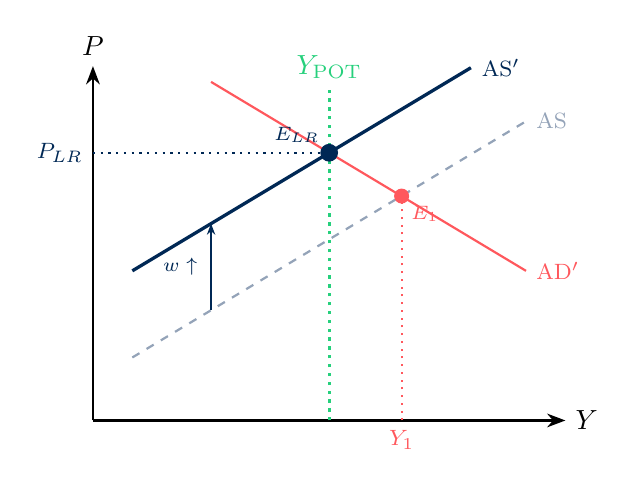
\begin{tikzpicture}[scale=1.0]
            % Axes
            \draw[-{Stealth}, thick] (0,0) -- (6,0) node[right] {$Y$};
            \draw[-{Stealth}, thick] (0,0) -- (0,4.5) node[above] {$P$};
            % Y_POT
            \draw[HECgreen, very thick, dotted] (3.0,0) -- (3.0,4.2)
               node[above] {$Y_{\text{POT}}$};
            % AS original (dashed): y = 0.6x + 0.5
            \draw[HECgray, dashed, thick] (0.5,0.8) -- (5.5,3.8)
               node[right, font=\footnotesize] {AS};
            % AD' (solid, the new demand): y = -0.6x + 5.2
            \draw[HECcoral, thick] (1.5,4.3) -- (5.5,1.9)
               node[right, font=\footnotesize] {AD$'$};
            % AS' shifted left: y = 0.6x + 1.6 (passes through Y_POT at P=3.4)
            \draw[HECnavy, very thick] (0.5,1.9) -- (4.8,4.48)
               node[right, font=\footnotesize] {AS$'$};
            % E1: AD' ∩ AS at (3.92, 2.85)
            \filldraw[HECcoral] (3.92,2.85) circle (2.5pt);
            \node[font=\scriptsize, HECcoral, below right] at (3.92,2.85) {$E_1$};
            % E_LR: AD' ∩ AS' at (3.0, 3.4)
            \filldraw[HECnavy] (3.0,3.4) circle (3pt);
            \node[font=\scriptsize, HECnavy, above left] at (3.0,3.4) {$E_{LR}$};
            % AS adjustment arrow (AS → AS')
            \draw[-{Stealth[length=4pt]}, HECnavy, thick] (1.5,1.4) -- (1.5,2.5);
            \node[font=\scriptsize, HECnavy, left] at (1.45,1.95) {$w\uparrow$};
            % Dotted reference lines
            \draw[dotted, thick, HECcoral] (3.92,0) node[below, font=\footnotesize] {$Y_1$} -- (3.92,2.85);
            \draw[dotted, thick, HECnavy] (0,3.4) node[left, font=\footnotesize] {$P_{LR}$} -- (3.0,3.4);
         \end{tikzpicture}
      \end{column}
      \begin{column}{0.42\textwidth}
         \small
         \textbf{Long terme :}
         \vspace{0.15cm}
         \begin{enumerate}
            \setlength\itemsep{0.1cm}
            \item $Y_1 > Y_{\text{POT}}$ $\to$ ch\^{o}mage faible
            \item Travailleurs rares
            \item Salaires nominaux $\uparrow$ $\to$ co\^{u}ts $\uparrow$
            \item AS se d\'{e}place vers la gauche
            \item Retour \`{a} $Y_{\text{POT}}$ au prix $P_{LR}$
         \end{enumerate}
         \vspace{0.2cm}
         \textcolor{HECgray}{\footnotesize M\^{e}me niveau de production, mais à un niveau de prix plus \'{e}lev\'{e}.}
      \end{column}
   \end{columns}
\end{frame}

\begin{frame}[t]{Pourquoi ne pas laisser la nature guérir d'elle-même\,?}
   \vspace{0.2cm}
   \begin{columns}[T]
      \begin{column}{0.47\textwidth}
         \textbf{\textcolor{HECnavy}{L'ajustement est lent}}
         \vspace{0.15cm}
         \begin{itemize}
            \setlength\itemsep{0.15cm}
            \item Prix : dur\'{e}e moyenne de 8 mois
            \item Salaires : dur\'{e}e moyenne d'1 an
            \item Ajustement complet : \textbf{2 \`{a} 3 ans}
         \end{itemize}
      \end{column}
      \begin{column}{0.47\textwidth}
         \textbf{\textcolor{HECcoral}{Les r\'{e}cessions sont co\^{u}teuses}}
         \vspace{0.15cm}
         \begin{itemize}
            \setlength\itemsep{0.15cm}
            \item Ch\^{o}mage massif, faillites
            \item Hyst\'{e}r\`{e}se : effets \textbf{permanents}
            \item Co\^{u}ts sociaux (sant\'{e}, criminalit\'{e})
         \end{itemize}
      \end{column}
   \end{columns}
   \vspace{0.3cm}
   \begin{keyinsight}[Diplômer en récession]
      
   \end{keyinsight}
\end{frame}

\tikzset{
   casebox/.style={rectangle, rounded corners=8pt, draw=#1, line width=0.8pt,
                   fill=#1!8, minimum width=3.2cm, minimum height=1cm,
                   align=center, font=\small, inner sep=5pt},
   casearr/.style={->, >=stealth, line width=1.2pt, #1},
}
\begin{frame}{2020--2022 : un cas d'\'{e}tude grandeur nature}
   \vspace{0.2cm}
   \centering
   \begin{tikzpicture}
      \node[casebox=HECnavy] (a) at (0,0) {\textbf{2020}\\Pand\'{e}mie};
      \node[casebox=HECgreen] (b) at (4.5,0) {\textbf{2020--21}\\Relance massive};
      \node[casebox=HECcoral] (c) at (9,0) {\textbf{2022}\\Inflation \`{a} 8\,\%};
      \draw[casearr=HECnavy] (a) -- (b);
      \draw[casearr=HECgreen] (b) -- (c);
   \end{tikzpicture}
   \vspace{0.3cm}
   \begin{keyinsight}
      La politique contracyclique a \'{e}vit\'{e} une d\'{e}pression majeure, mais la relance \'{e}tait-elle \textbf{trop g\'{e}n\'{e}reuse}\,? Comprendre ces outils et leurs limites, c'est le c\oe ur de cette s\'{e}ance.
   \end{keyinsight}
\end{frame}

\begin{frame}[t]{Deux institutions, deux leviers}
   \vspace{0.3cm}
   \begin{columns}[T]
      \begin{column}{0.47\textwidth}
         \centering
         \textcolor{HECnavy}{\large\textbf{Politique mon\'{e}taire}}\\[3pt]
         \textcolor{HECgray}{Banque centrale}\\[8pt]
         \small
         \begin{itemize}
            \setlength\itemsep{0.15cm}
            \item Taux d'int\'{e}r\^{e}t directeur
            \item D\'{e}cision rapide (8 annonces/an)
            \item \textbf{Ind\'{e}pendante} du gouvernement
            \item Agit sur AD via $C$ et $I$
         \end{itemize}
      \end{column}
      \begin{column}{0.06\textwidth}
         \centering
         \vspace{0.8cm}
         {\Large\textcolor{HECgray}{vs.\,}}
      \end{column}
      \begin{column}{0.47\textwidth}
         \centering
         \textcolor{HECgreen}{\large\textbf{Politique budg\'{e}taire}}\\[3pt]
         \textcolor{HECgray}{Gouvernement}\\[8pt]
         \small
         \begin{itemize}
            \setlength\itemsep{0.15cm}
            \item D\'{e}penses ($G$), imp\^{o}ts ($T$), transferts
            \item Processus l\'{e}gislatif (lent)
            \item D\'{e}cision \textbf{politique}
            \item Agit sur AD via $G$, $C$ et $I$
         \end{itemize}
      \end{column}
   \end{columns}
\end{frame}

% ============================================================================

\begin{frame}{Plan}
   \begin{enumerate}
      \setlength\itemsep{0.5cm}
      \item {\color{gray!50}Pourquoi combattre les r\'{e}cessions\,?}
      \item \textbf{La politique mon\'{e}taire conventionnelle}
      \item D\'{e}fis et limites de la politique mon\'{e}taire
      \item La politique mon\'{e}taire non conventionnelle
      \item La politique budg\'{e}taire
      \item La dette publique
   \end{enumerate}
\end{frame}

% ============================================================================
\sectionframe{La politique mon\'{e}taire conventionnelle}
% ============================================================================

\begin{frame}[t]{La Banque du Canada : r\^{o}les}
   \small
   \vspace{0.2cm}
   \begin{enumerate}
      \setlength\itemsep{0.25cm}
      \item \textbf{Politique mon\'{e}taire} --- maintenir l'inflation basse, stable et pr\'{e}visible
      \item \textbf{Stabilit\'{e} financi\`{e}re} --- partenariat avec les organismes de r\'{e}glementation
      \item \textbf{\'{E}mission de la monnaie} --- conception et \'{e}mission des billets de banque
      \item \textbf{Gestion financi\`{e}re} --- tr\'{e}sorier du gouvernement f\'{e}d\'{e}ral
      \item \textbf{Syst\`{e}mes de paiement} --- surveillance de l'infrastructure de paiement
   \end{enumerate}
   \vspace{0.2cm}
   \begin{keyinsight}[Ind\'{e}pendance]
      La BdC est une institution publique \textbf{ind\'{e}pendante} du gouvernement sur le plan op\'{e}rationnel. C'est cette ind\'{e}pendance qui fonde sa \textbf{cr\'{e}dibilit\'{e}}.
   \end{keyinsight}
\end{frame}

\begin{frame}[t]{La cible d'inflation : 2\,\%}
   \small
   \vspace{0.2cm}
   \begin{defbox}[Entente BdC--Gouvernement]
      Cible de \textbf{2\,\%} d'inflation (IPC), avec une fourchette de \textbf{1 \`{a} 3\,\%}. Renouvel\'{e}e tous les 5 ans (derni\`{e}re fois en 2021).
   \end{defbox}
   \vspace{0.15cm}
   \textbf{Pourquoi 2\,\% et non 0\,\%\,?}
   \vspace{0.1cm}
   \begin{itemize}
      \setlength\itemsep{0.15cm}
      \item La \textbf{d\'{e}flation} est pire que l'inflation mod\'{e}r\'{e}e (spirale d\'{e}flationniste)
      \item \textbf{Rigidit\'{e} nominale} des salaires : les employeurs ne peuvent pas facilement baisser les salaires nominaux. L'inflation permet un ajustement \guillemotleft~silencieux~\guillemotright\ des salaires r\'{e}els.
      \item \textbf{Marge de man\oe uvre} : permet de baisser les taux r\'{e}els en territoire n\'{e}gatif si n\'{e}cessaire
   \end{itemize}
\end{frame}

\begin{frame}[t]{L'instrument : le taux directeur}
   \small
   \vspace{0.15cm}
   \begin{defbox}[Taux directeur (taux \`{a} un jour)]
      Le taux auquel les grandes banques commerciales s'\'{e}changent des fonds pour une \textbf{journ\'{e}e}.
   \end{defbox}
   \vspace{0.05cm}
   \begin{itemize}
      \setlength\itemsep{0.12cm}
      \item La BdC annonce une \textbf{cible} pour ce taux, 8 fois par ann\'{e}e (dates fixes)
      \item Elle l'atteint en ajustant l'\textbf{offre de liquidit\'{e}s} dans le syst\`{e}me bancaire
      \item Actuellement : \textbf{2.25\,\%} (mars 2026)
   \end{itemize}
   \vspace{0.05cm}
   \begin{bizimplication}
      Quand la BdC baisse le taux, votre marge de cr\'{e}dit co\^{u}te moins cher \textbf{le lendemain}. L'hypoth\`{e}que suit en quelques semaines.
   \end{bizimplication}
\end{frame}

\begin{frame}[t]{Le march\'{e} interbancaire \`{a} un jour}
   \small
   \vspace{0.2cm}
   \textbf{Pourquoi les banques s'empruntent-elles de l'argent chaque nuit\,?}
   \vspace{0.15cm}
   \begin{itemize}
      \setlength\itemsep{0.15cm}
      \item Chaque jour, des millions de transactions entre clients de banques diff\'{e}rentes
      \item En fin de journ\'{e}e : certaines banques ont un \textbf{surplus} de liquidit\'{e}s, d'autres un \textbf{d\'{e}ficit}
      \item Les banques en surplus \textbf{pr\^{e}tent} \`{a} celles en d\'{e}ficit pour \textbf{une nuit}
      \item Le taux de ce pr\^{e}t = \textbf{taux \`{a} un jour} (\textit{overnight rate})
   \end{itemize}
   \vspace{0.15cm}
   \begin{bizimplication}
      La BdC contr\^{o}le ce taux en ajustant l'offre de liquidit\'{e}s dans le syst\`{e}me. Plus de liquidit\'{e}s $\to$ surplus $\uparrow$ $\to$ prix de l'emprunt $\downarrow$ $\to$ taux \`{a} un jour $\downarrow$.
   \end{bizimplication}
\end{frame}

\begin{frame}{Le syst\`{e}me de corridor}
   \centering
   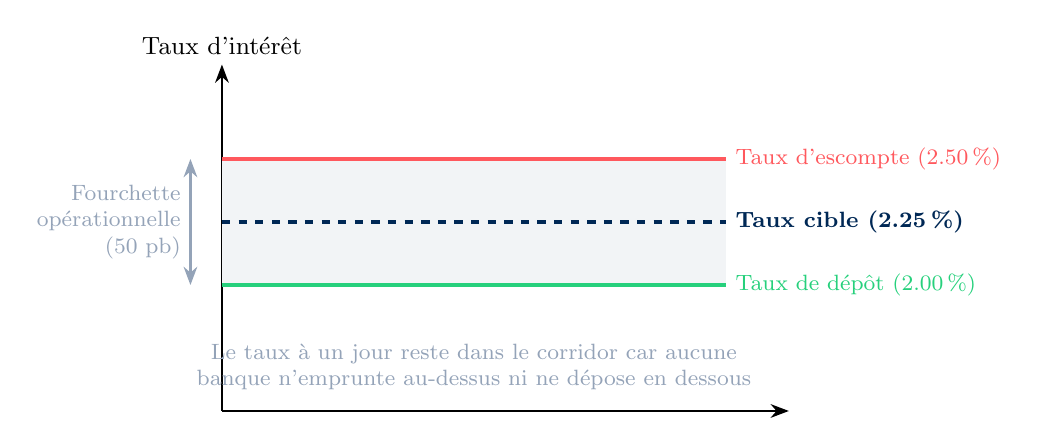
\begin{tikzpicture}[scale=0.80]
      % Axes
      \draw[-{Stealth}, thick] (0,0) -- (9,0) node[right] {};
      \draw[-{Stealth}, thick] (0,0) -- (0,5.5) node[above, font=\small] {Taux d'int\'{e}r\^{e}t};
      % Corridor shading
      \fill[HECnavy!5] (0,2.0) rectangle (8.0,4.0);
      % Bank rate (ceiling)
      \draw[HECcoral, very thick] (0,4.0) -- (8.0,4.0);
      \node[right, font=\footnotesize, HECcoral] at (8.0,4.0) {Taux d'escompte (2.50\,\%)};
      % Target rate (middle)
      \draw[HECnavy, very thick, dashed] (0,3.0) -- (8.0,3.0);
      \node[right, font=\footnotesize\bfseries, HECnavy] at (8.0,3.0) {Taux cible (2.25\,\%)};
      % Deposit rate (floor)
      \draw[HECgreen, very thick] (0,2.0) -- (8.0,2.0);
      \node[right, font=\footnotesize, HECgreen] at (8.0,2.0) {Taux de d\'{e}p\^{o}t (2.00\,\%)};
      % Annotations
      \draw[{Stealth}-{Stealth}, thick, HECgray] (-0.5,2.0) -- (-0.5,4.0);
      \node[left, font=\footnotesize, HECgray, align=right] at (-0.5,3.0) {Fourchette\\op\'{e}rationnelle\\(50 pb)};
      % Labels
      \node[font=\footnotesize, HECgray, align=center, text width=8cm] at (4.0,0.7) {Le taux \`{a} un jour reste dans le corridor car aucune\\banque n'emprunte au-dessus ni ne d\'{e}pose en dessous};
   \end{tikzpicture}
\end{frame}

\begin{frame}{Le taux directeur depuis 1996}
   \begin{figure}
      \centering
      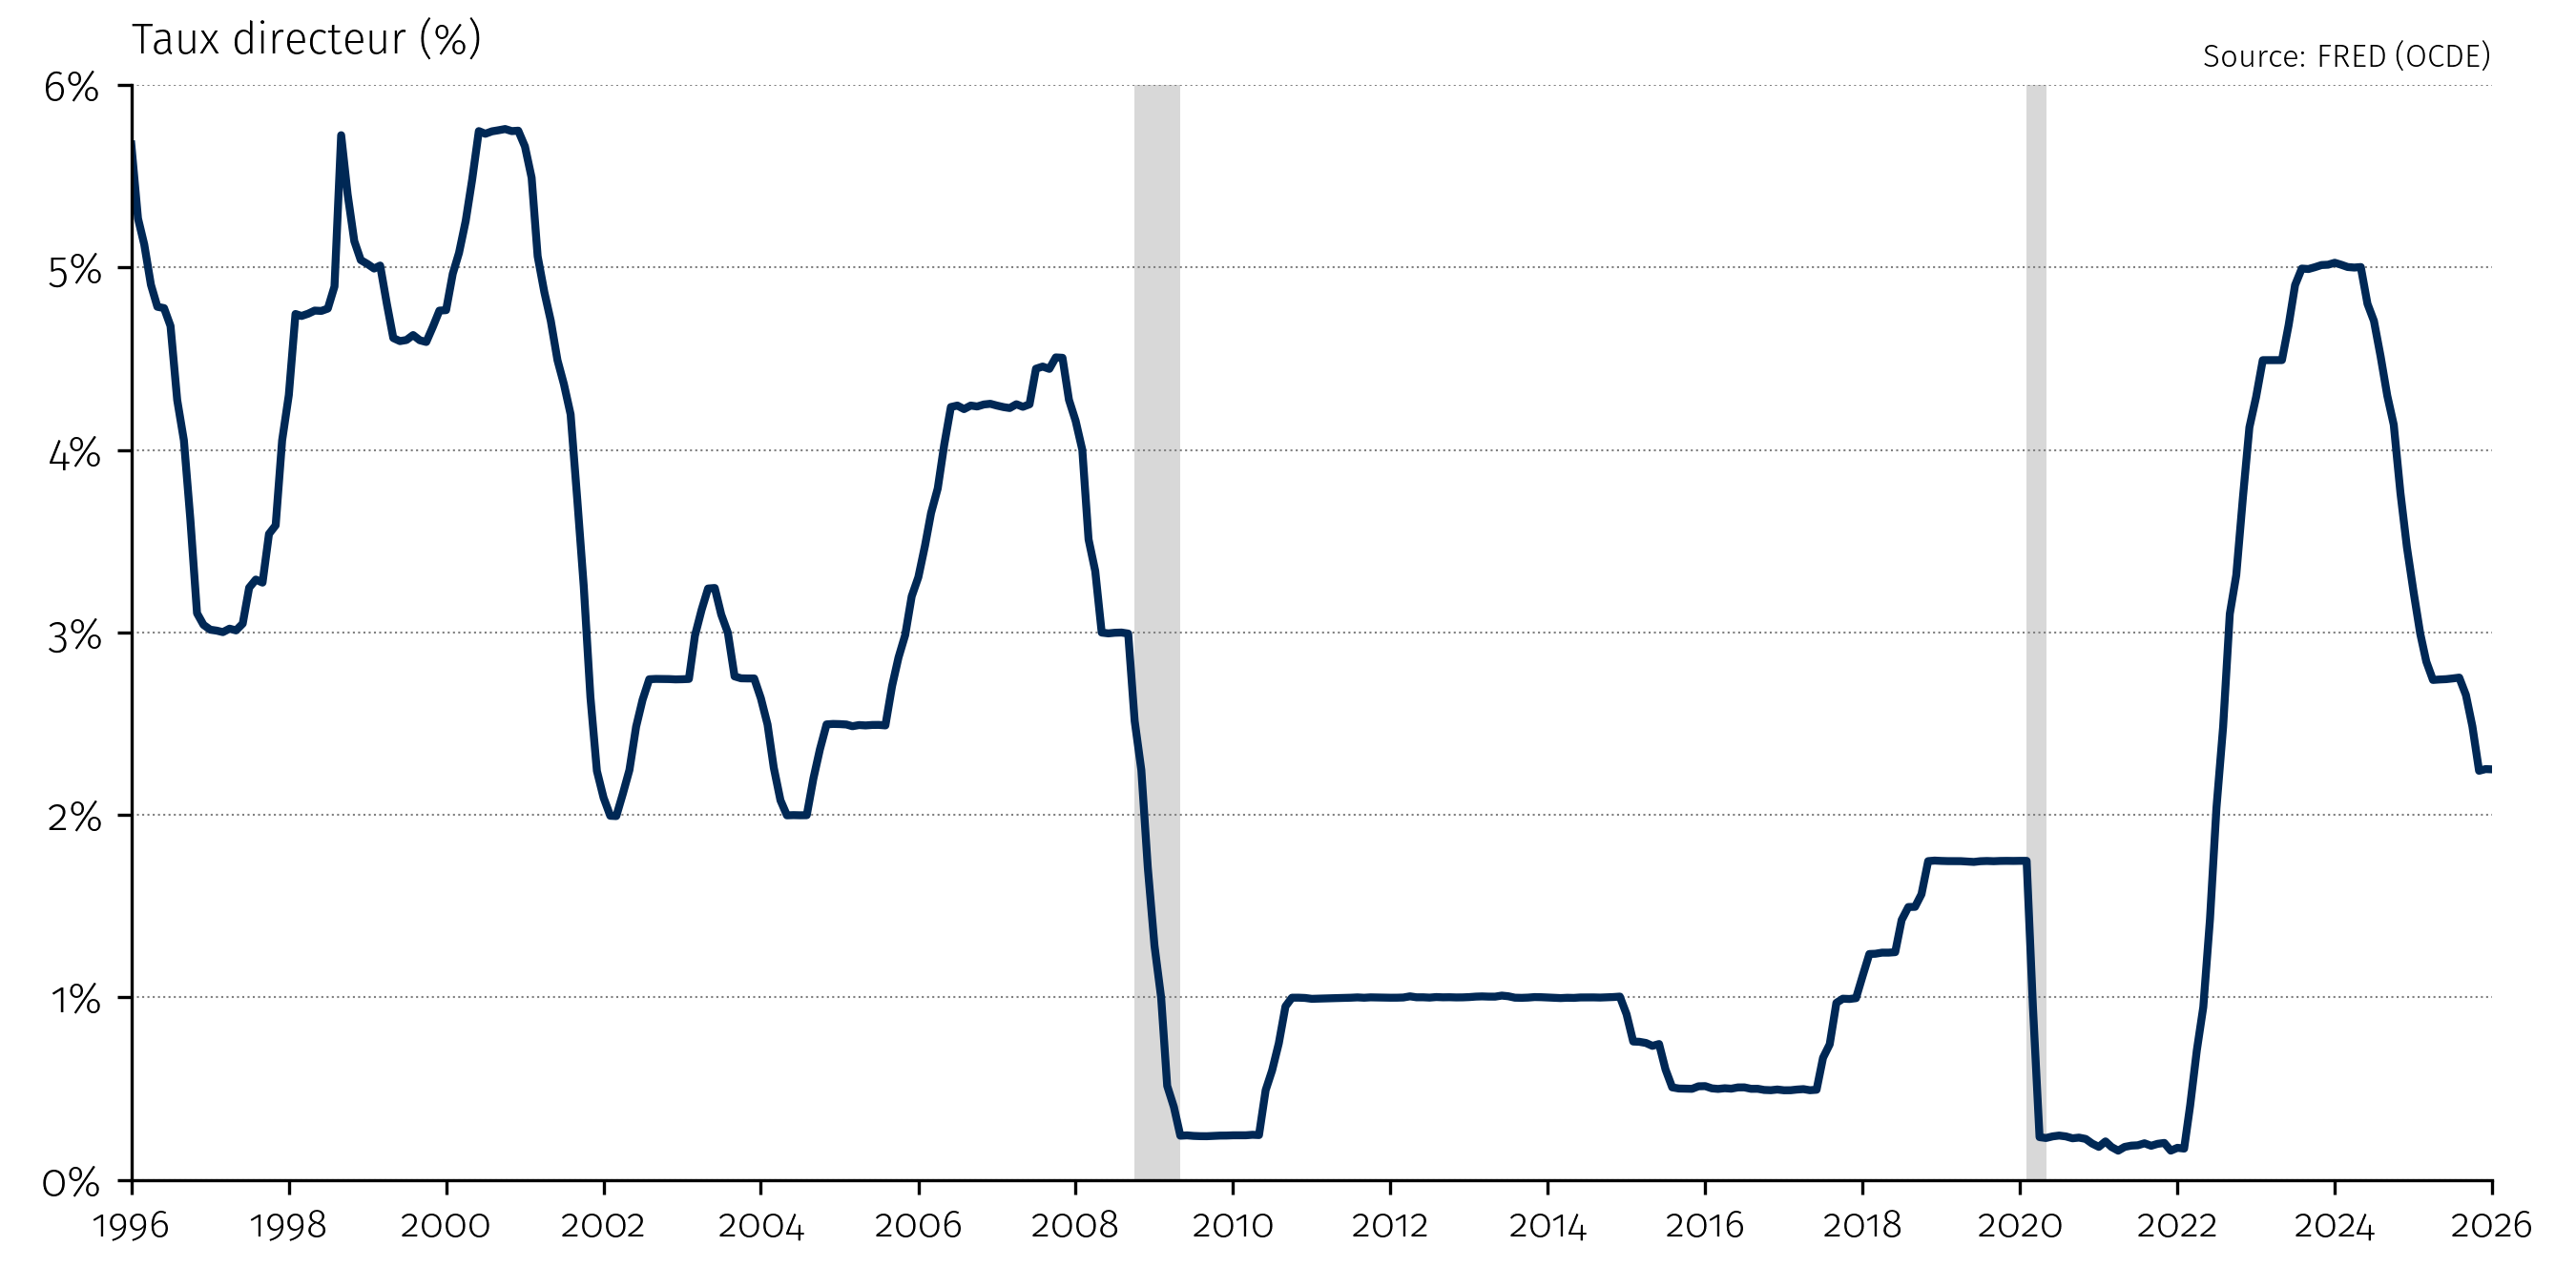
\includegraphics[width=0.95\textwidth, height=0.78\textheight, keepaspectratio]{overnight_rate_ca.png}
   \end{figure}
\end{frame}

\begin{frame}[t]{Politique expansionniste : $\downarrow$ taux $\to$ $\uparrow$ AD}
   \small
   \vspace{0.1cm}
   \textbf{M\'{e}canisme :} BdC $\downarrow$ taux directeur $\to$ taux du march\'{e} $\downarrow$
   \vspace{0.1cm}
   \begin{itemize}
      \setlength\itemsep{0.1cm}
      \item $C \uparrow$ : pr\^{e}ts automobiles, hypoth\`{e}ques moins co\^{u}teux
      \item $I \uparrow$ : co\^{u}t d'emprunt des entreprises $\downarrow$ $\to$ plus de projets rentables
      \item $NX \uparrow$ : taux $\downarrow$ $\to$ dollar $\downarrow$ $\to$ exportations plus comp\'{e}titives
   \end{itemize}
   \vspace{0.05cm}
   \centering
   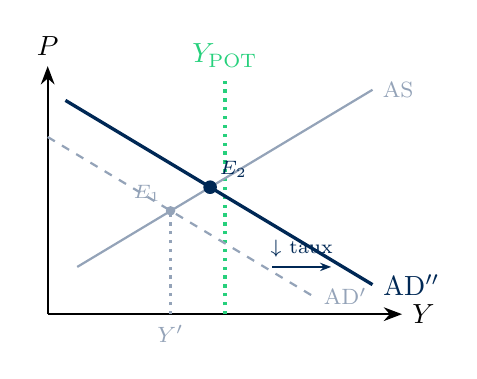
\begin{tikzpicture}[scale=0.75]
      % Axes
      \draw[-{Stealth}, thick] (0,0) -- (6,0) node[right] {$Y$};
      \draw[-{Stealth}, thick] (0,0) -- (0,4.2) node[above] {$P$};
      % Y_POT
      \draw[HECgreen, very thick, dotted] (3.0,0) -- (3.0,4.0)
         node[above] {$Y_{\text{POT}}$};
      % AS: y = 0.6x + 0.5
      \draw[HECgray, thick] (0.5,0.8) -- (5.5,3.8)
         node[right, font=\footnotesize] {AS};
      % AD' (recession): y = -0.6x + 3.0
      \draw[HECgray, dashed, thick] (0.0,3.0) -- (4.5,0.3)
         node[right, font=\footnotesize] {AD$'$};
      % AD'' (after policy): y = -0.6x + 3.8
      \draw[HECnavy, very thick] (0.3,3.62) -- (5.5,0.5)
         node[right] {AD$''$};
      % Policy arrow at y=0.8: AD' at x=3.67, AD'' at x=5.0
      \draw[-{Stealth[length=4pt]}, HECnavy, thick] (3.8,0.8) -- (4.8,0.8);
      \node[font=\scriptsize, HECnavy, above] at (4.3,0.8) {$\downarrow$ taux};
      % Equilibria
      \filldraw[HECgray] (2.08,1.75) circle (2pt);
      \node[font=\scriptsize, HECgray, above left] at (2.08,1.75) {$E_1$};
      \filldraw[HECnavy] (2.75,2.15) circle (3pt);
      \node[font=\scriptsize, HECnavy, above right] at (2.75,2.15) {$E_2$};
      \draw[dotted, very thick, HECgray] (2.08,0) node[below, font=\footnotesize] {$Y'$} -- (2.08,1.75);
   \end{tikzpicture}
\end{frame}

\begin{frame}{Le m\'{e}canisme de transmission}
   \centering
   \vspace{0.3cm}
   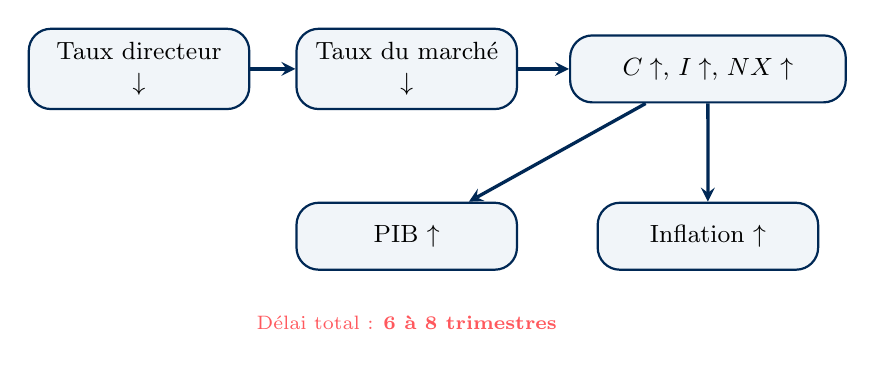
\begin{tikzpicture}[scale=0.85,
      box/.style={rectangle, rounded corners=8pt, draw=HECnavy, line width=0.8pt,
                  fill=HEClightgray, minimum width=2.8cm, minimum height=0.85cm,
                  align=center, font=\small, inner sep=5pt},
      arr/.style={->, HECnavy, >=stealth, line width=1.2pt}]
      % Row 1: policy transmission
      \node[box] (td) at (0,0) {Taux directeur\\$\downarrow$};
      \node[box] (tm) at (4,0) {Taux du march\'{e}\\$\downarrow$};
      \node[box, minimum width=3.5cm] (dec) at (8.5,0) {$C\uparrow$, $I\uparrow$, $NX\uparrow$};
      % Row 2: outcomes
      \node[box] (pib) at (4,-2.5) {PIB $\uparrow$};
      \node[box] (inf) at (8.5,-2.5) {Inflation $\uparrow$};
      % Arrows
      \draw[arr] (td) -- (tm);
      \draw[arr] (tm) -- (dec);
      \draw[arr] (dec) -- (pib);
      \draw[arr] (dec) -- (inf);
      % Delay annotation
      \node[font=\scriptsize, HECcoral, align=center] at (4,-3.8) {D\'{e}lai total : \textbf{6 \`{a} 8 trimestres}};
   \end{tikzpicture}
\end{frame}

\begin{frame}{Taux directeur et taux hypoth\'{e}caire}
   \begin{figure}
      \centering
      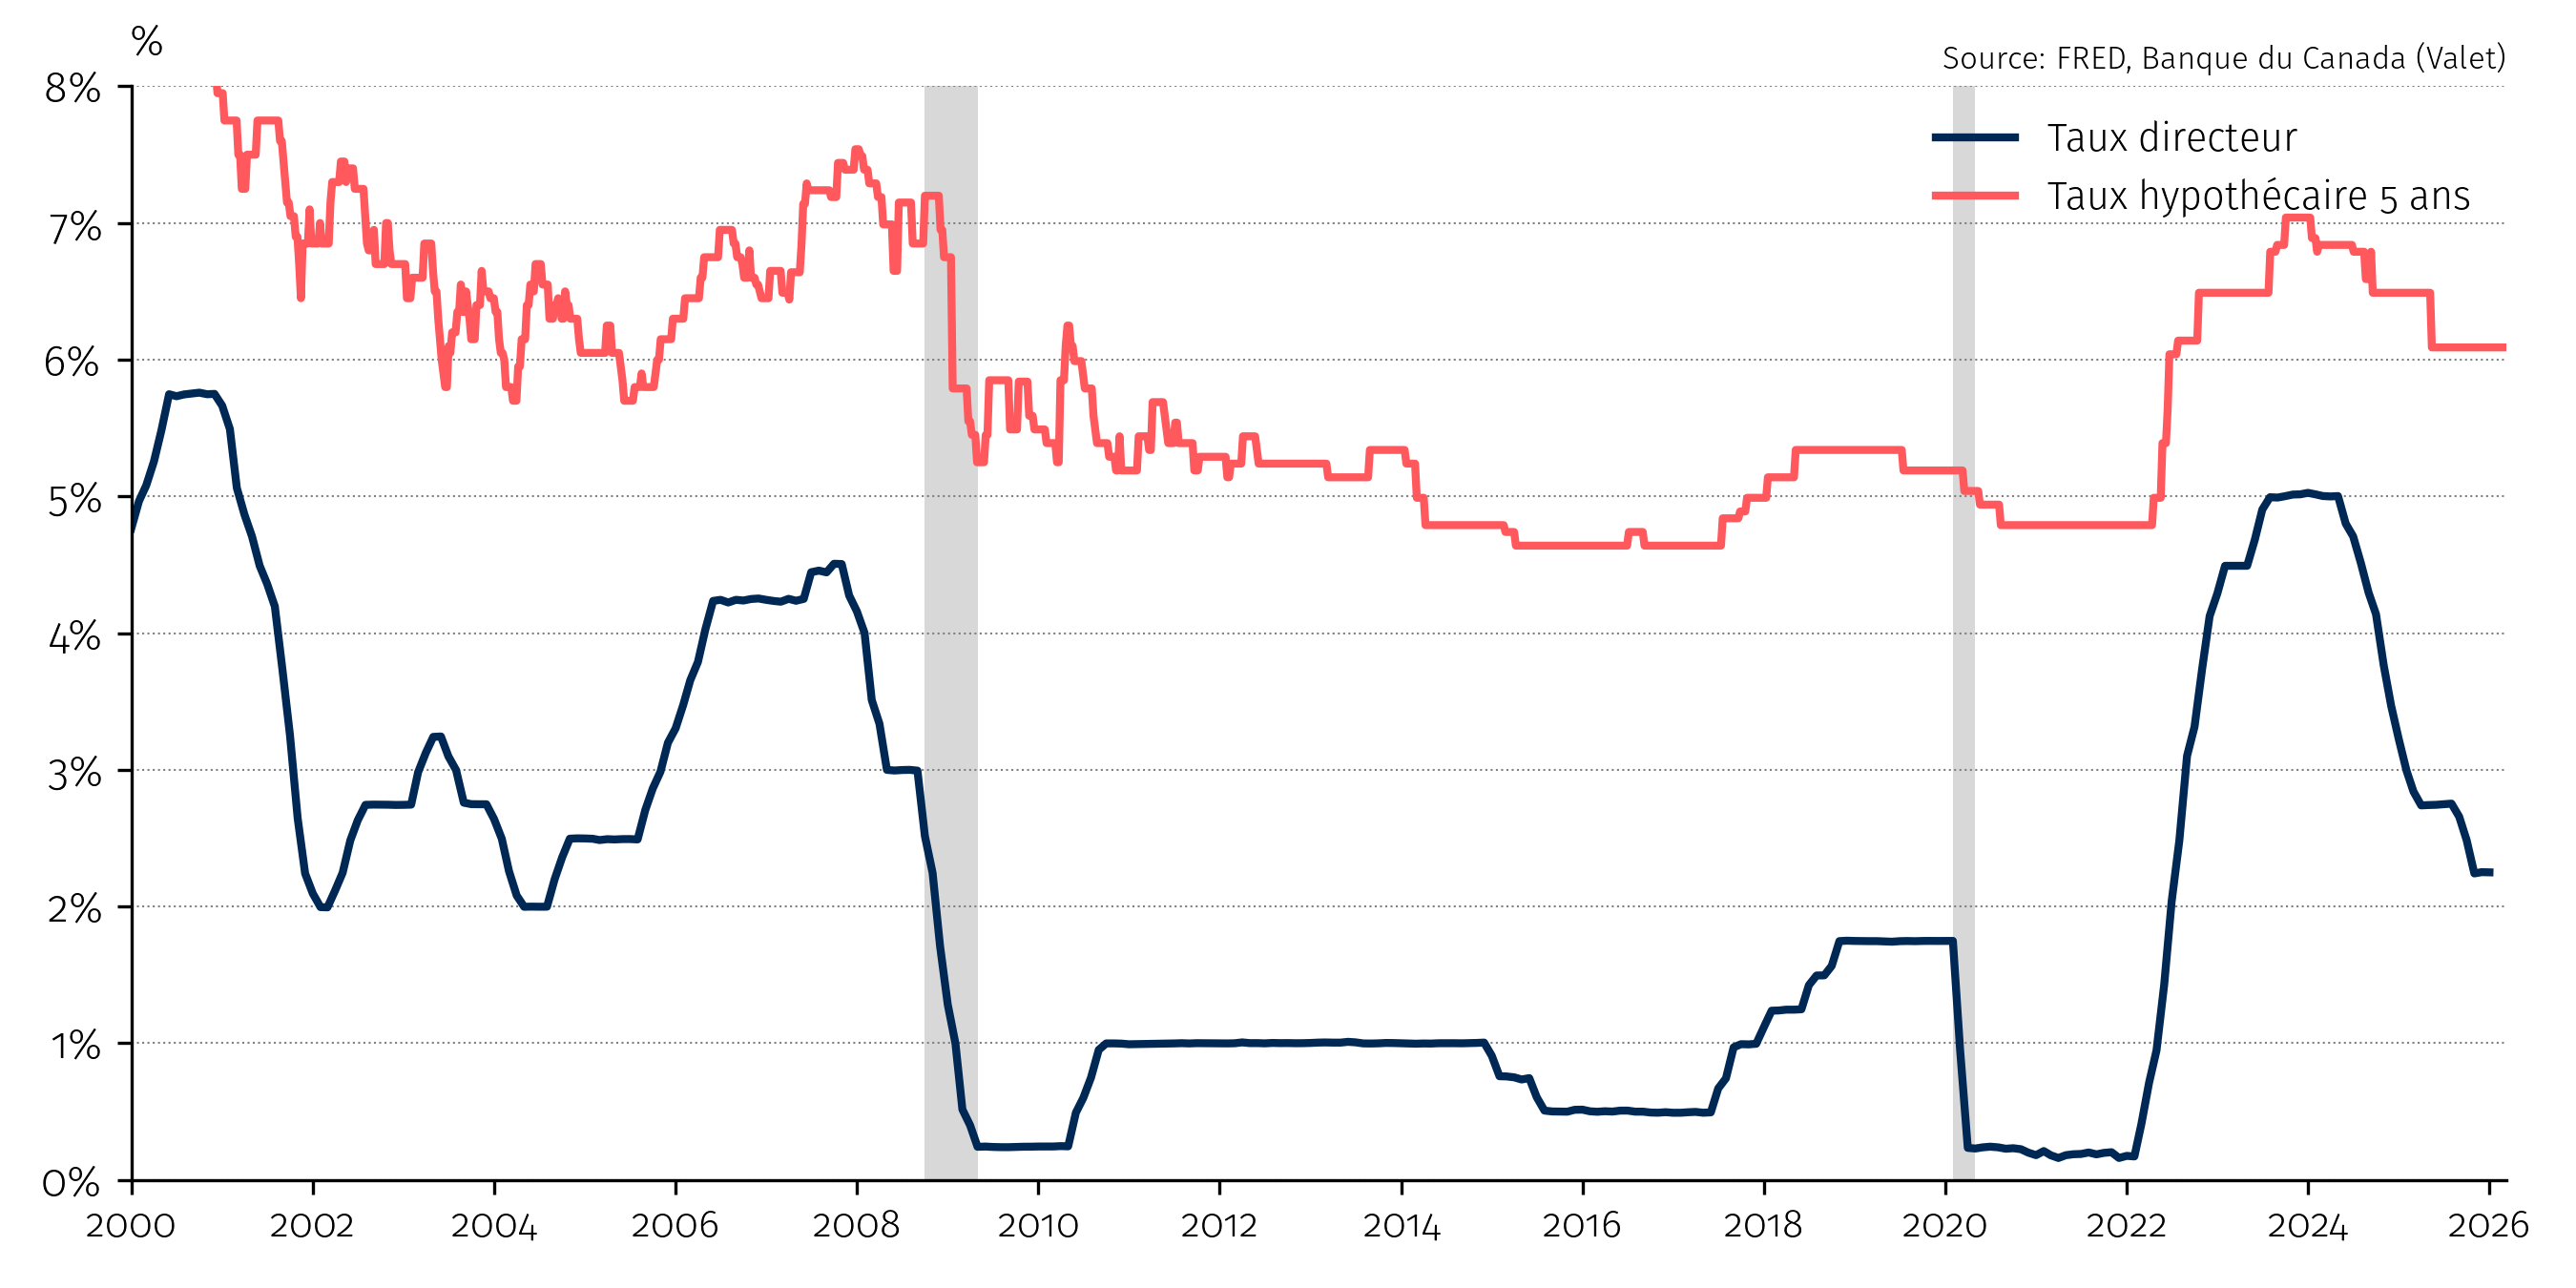
\includegraphics[width=0.95\textwidth, height=0.78\textheight, keepaspectratio]{overnight_vs_mortgage.png}
   \end{figure}
\end{frame}

\begin{frame}{Taux directeur et inflation (Canada)}
   \begin{figure}
      \centering
      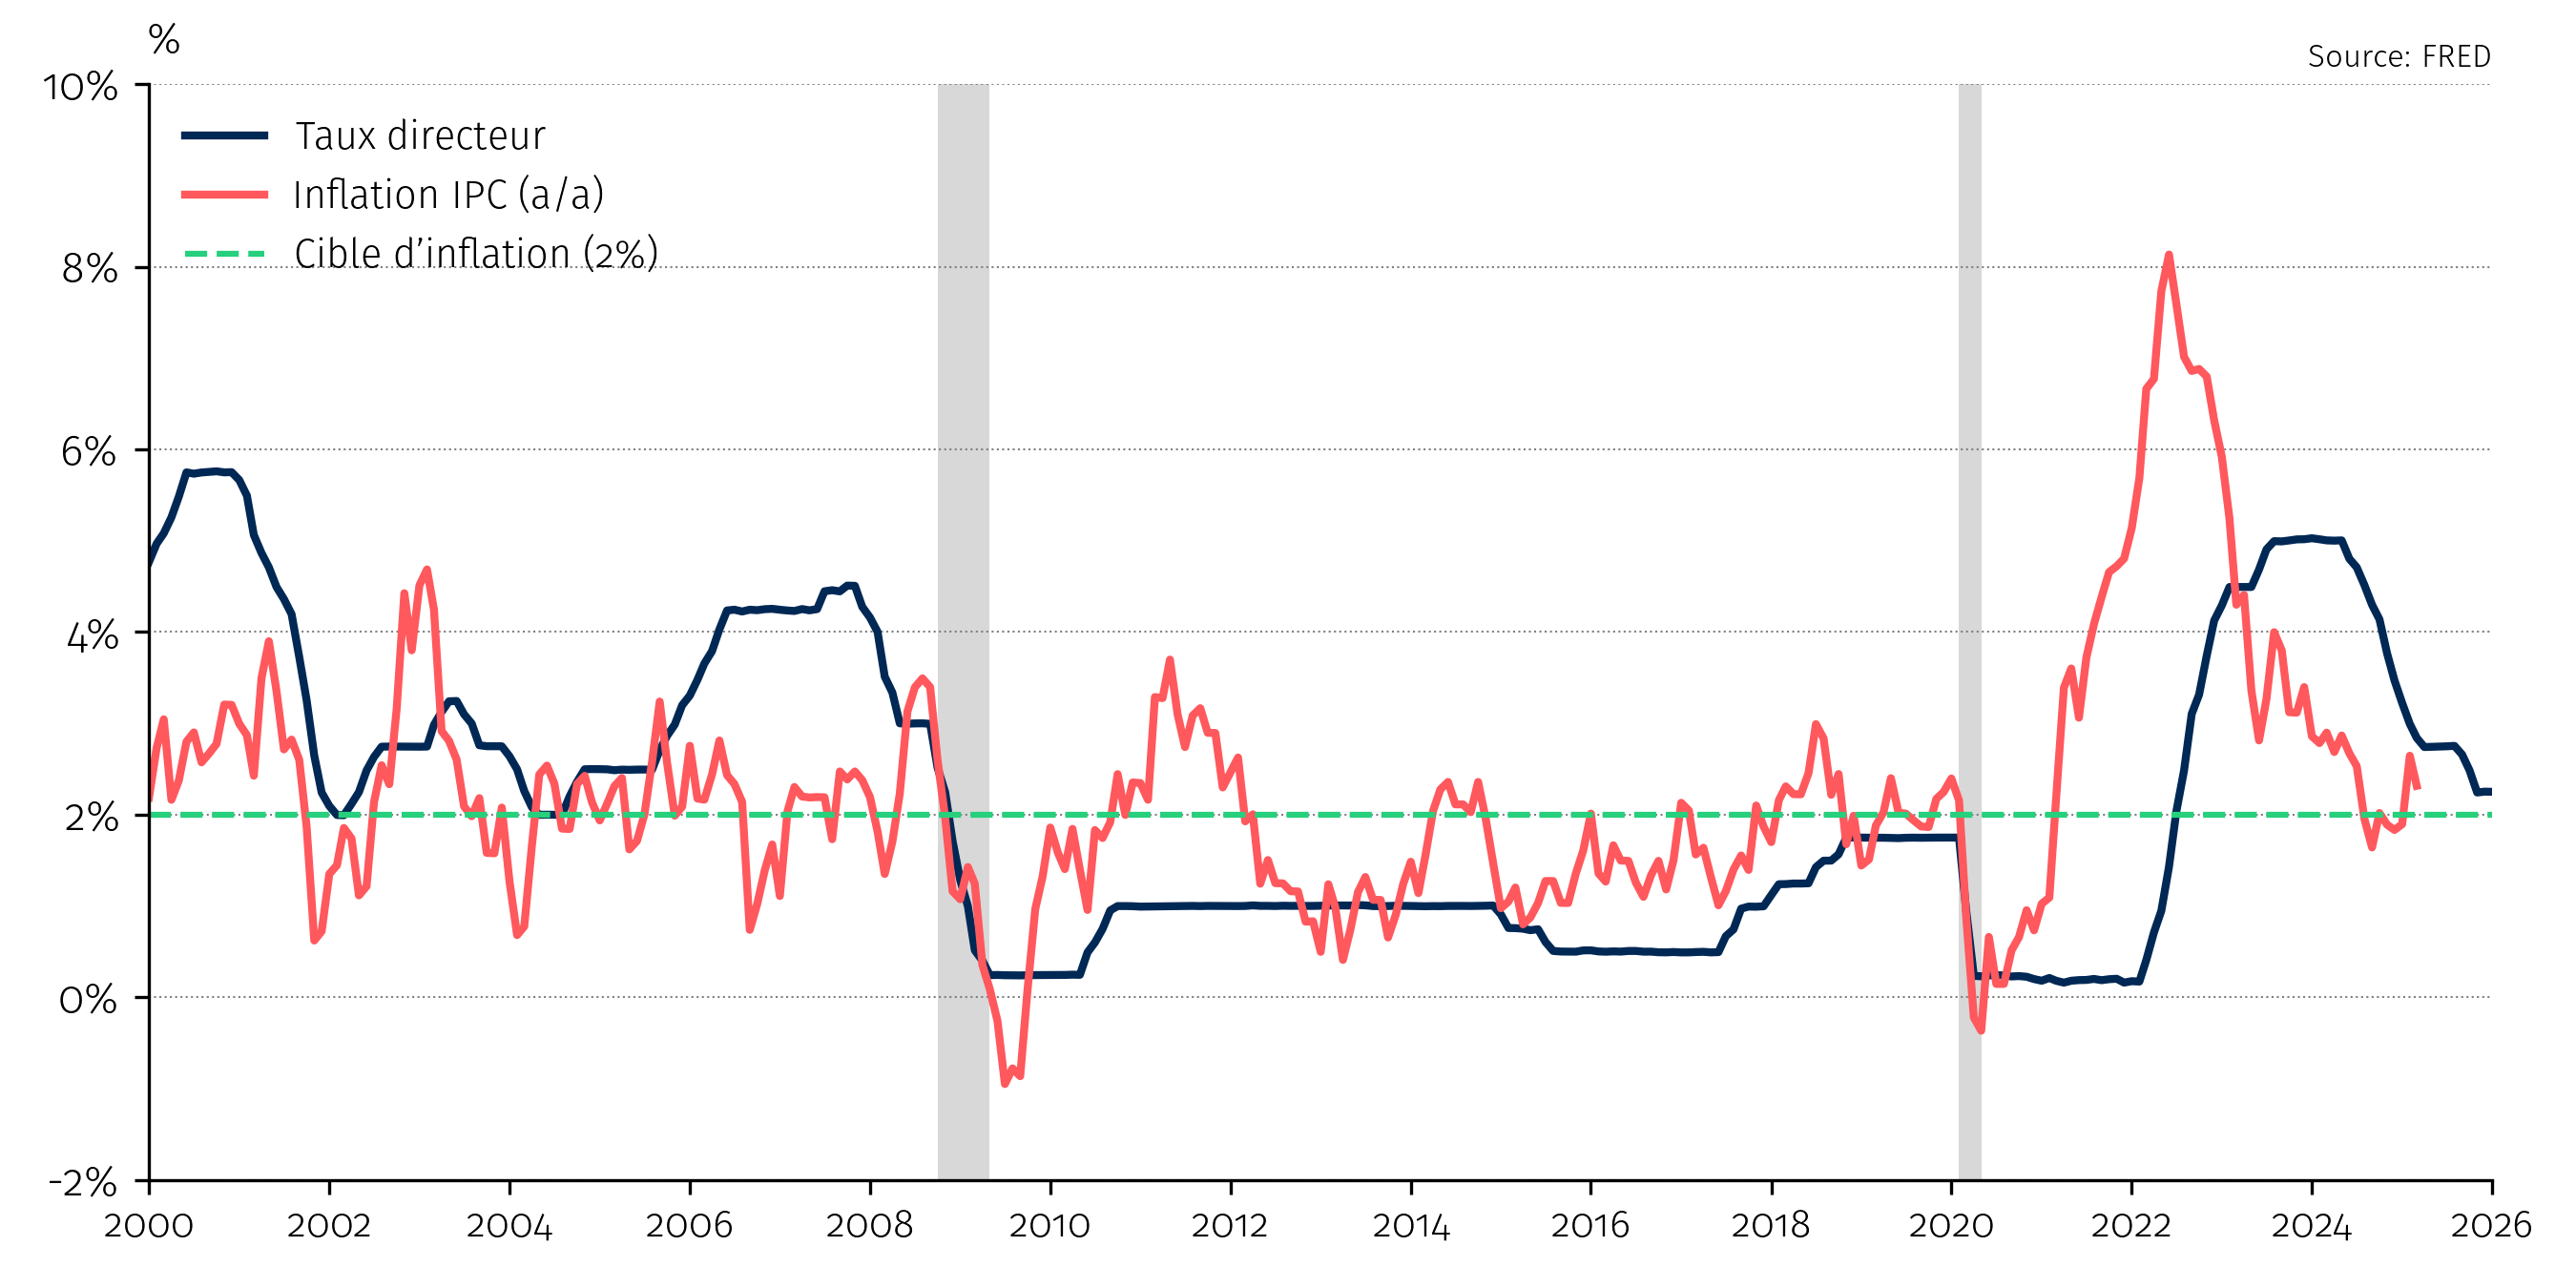
\includegraphics[width=0.95\textwidth, height=0.78\textheight, keepaspectratio]{rate_vs_inflation_ca.png}
   \end{figure}
\end{frame}

% ============================================================================

\begin{frame}{Plan}
   \begin{enumerate}
      \setlength\itemsep{0.5cm}
      \item {\color{gray!50}Pourquoi combattre les r\'{e}cessions\,?}
      \item {\color{gray!50}La politique mon\'{e}taire conventionnelle}
      \item \textbf{D\'{e}fis et limites de la politique mon\'{e}taire}
      \item La politique mon\'{e}taire non conventionnelle
      \item La politique budg\'{e}taire
      \item La dette publique
   \end{enumerate}
\end{frame}

% ============================================================================
\sectionframe{D\'{e}fis et limites de la politique mon\'{e}taire}
% ============================================================================

\begin{frame}[t]{D\'{e}fi 1 : l'incertitude}
   \small
   \vspace{0.2cm}
   \textbf{$Y_{\text{POT}}$ n'est pas directement observable.} Il faut l'\textbf{estimer}.
   \vspace{0.2cm}
   \begin{itemize}
      \setlength\itemsep{0.2cm}
      \item Quelle est la taille de l'\textbf{\'{e}cart de production}\,?
      \item L'\'{e}conomie est-elle en r\'{e}cession ou simplement en \textbf{ralentissement}\,?
      \item Les donn\'{e}es arrivent avec \textbf{retard} et sont souvent \textbf{r\'{e}vis\'{e}es}
   \end{itemize}
   \vspace{0.2cm}
   \begin{warning}
      Imaginez un m\'{e}decin qui prescrit un traitement sans conna\^{i}tre la temp\'{e}rature exacte du patient. C'est la r\'{e}alit\'{e} quotidienne d'un banquier central.
   \end{warning}
\end{frame}

\begin{frame}[t]{D\'{e}fi 2 : les d\'{e}lais de transmission}
   \small
   \vspace{0.2cm}
   \textbf{Consensus :} 6 \`{a} 8 trimestres entre la d\'{e}cision et l'effet maximal sur l'inflation.
   \vspace{0.2cm}
   \begin{itemize}
      \setlength\itemsep{0.2cm}
      \item La BdC doit donc agir en fonction de ses \textbf{pr\'{e}visions}, pas de la situation actuelle
      \item Les pr\'{e}visions sont \textbf{imparfaites} --- c'est loin d'\^{e}tre une science exacte
      \item M\'{e}taphore : \guillemotleft~conduire en regardant dans le r\'{e}troviseur~\guillemotright
   \end{itemize}
   \vspace{0.2cm}
   \begin{keyinsight}
      C'est pour cette raison que les banques centrales r\'{e}p\`{e}tent que leurs d\'{e}cisions sont \guillemotleft~\textit{forward-looking}~\guillemotright\ et d\'{e}pendent des \guillemotleft~donn\'{e}es \`{a} venir~\guillemotright.
   \end{keyinsight}
\end{frame}

\begin{frame}{L'erreur de 2021--22 : trop bas, trop longtemps}
   \begin{figure}
      \centering
      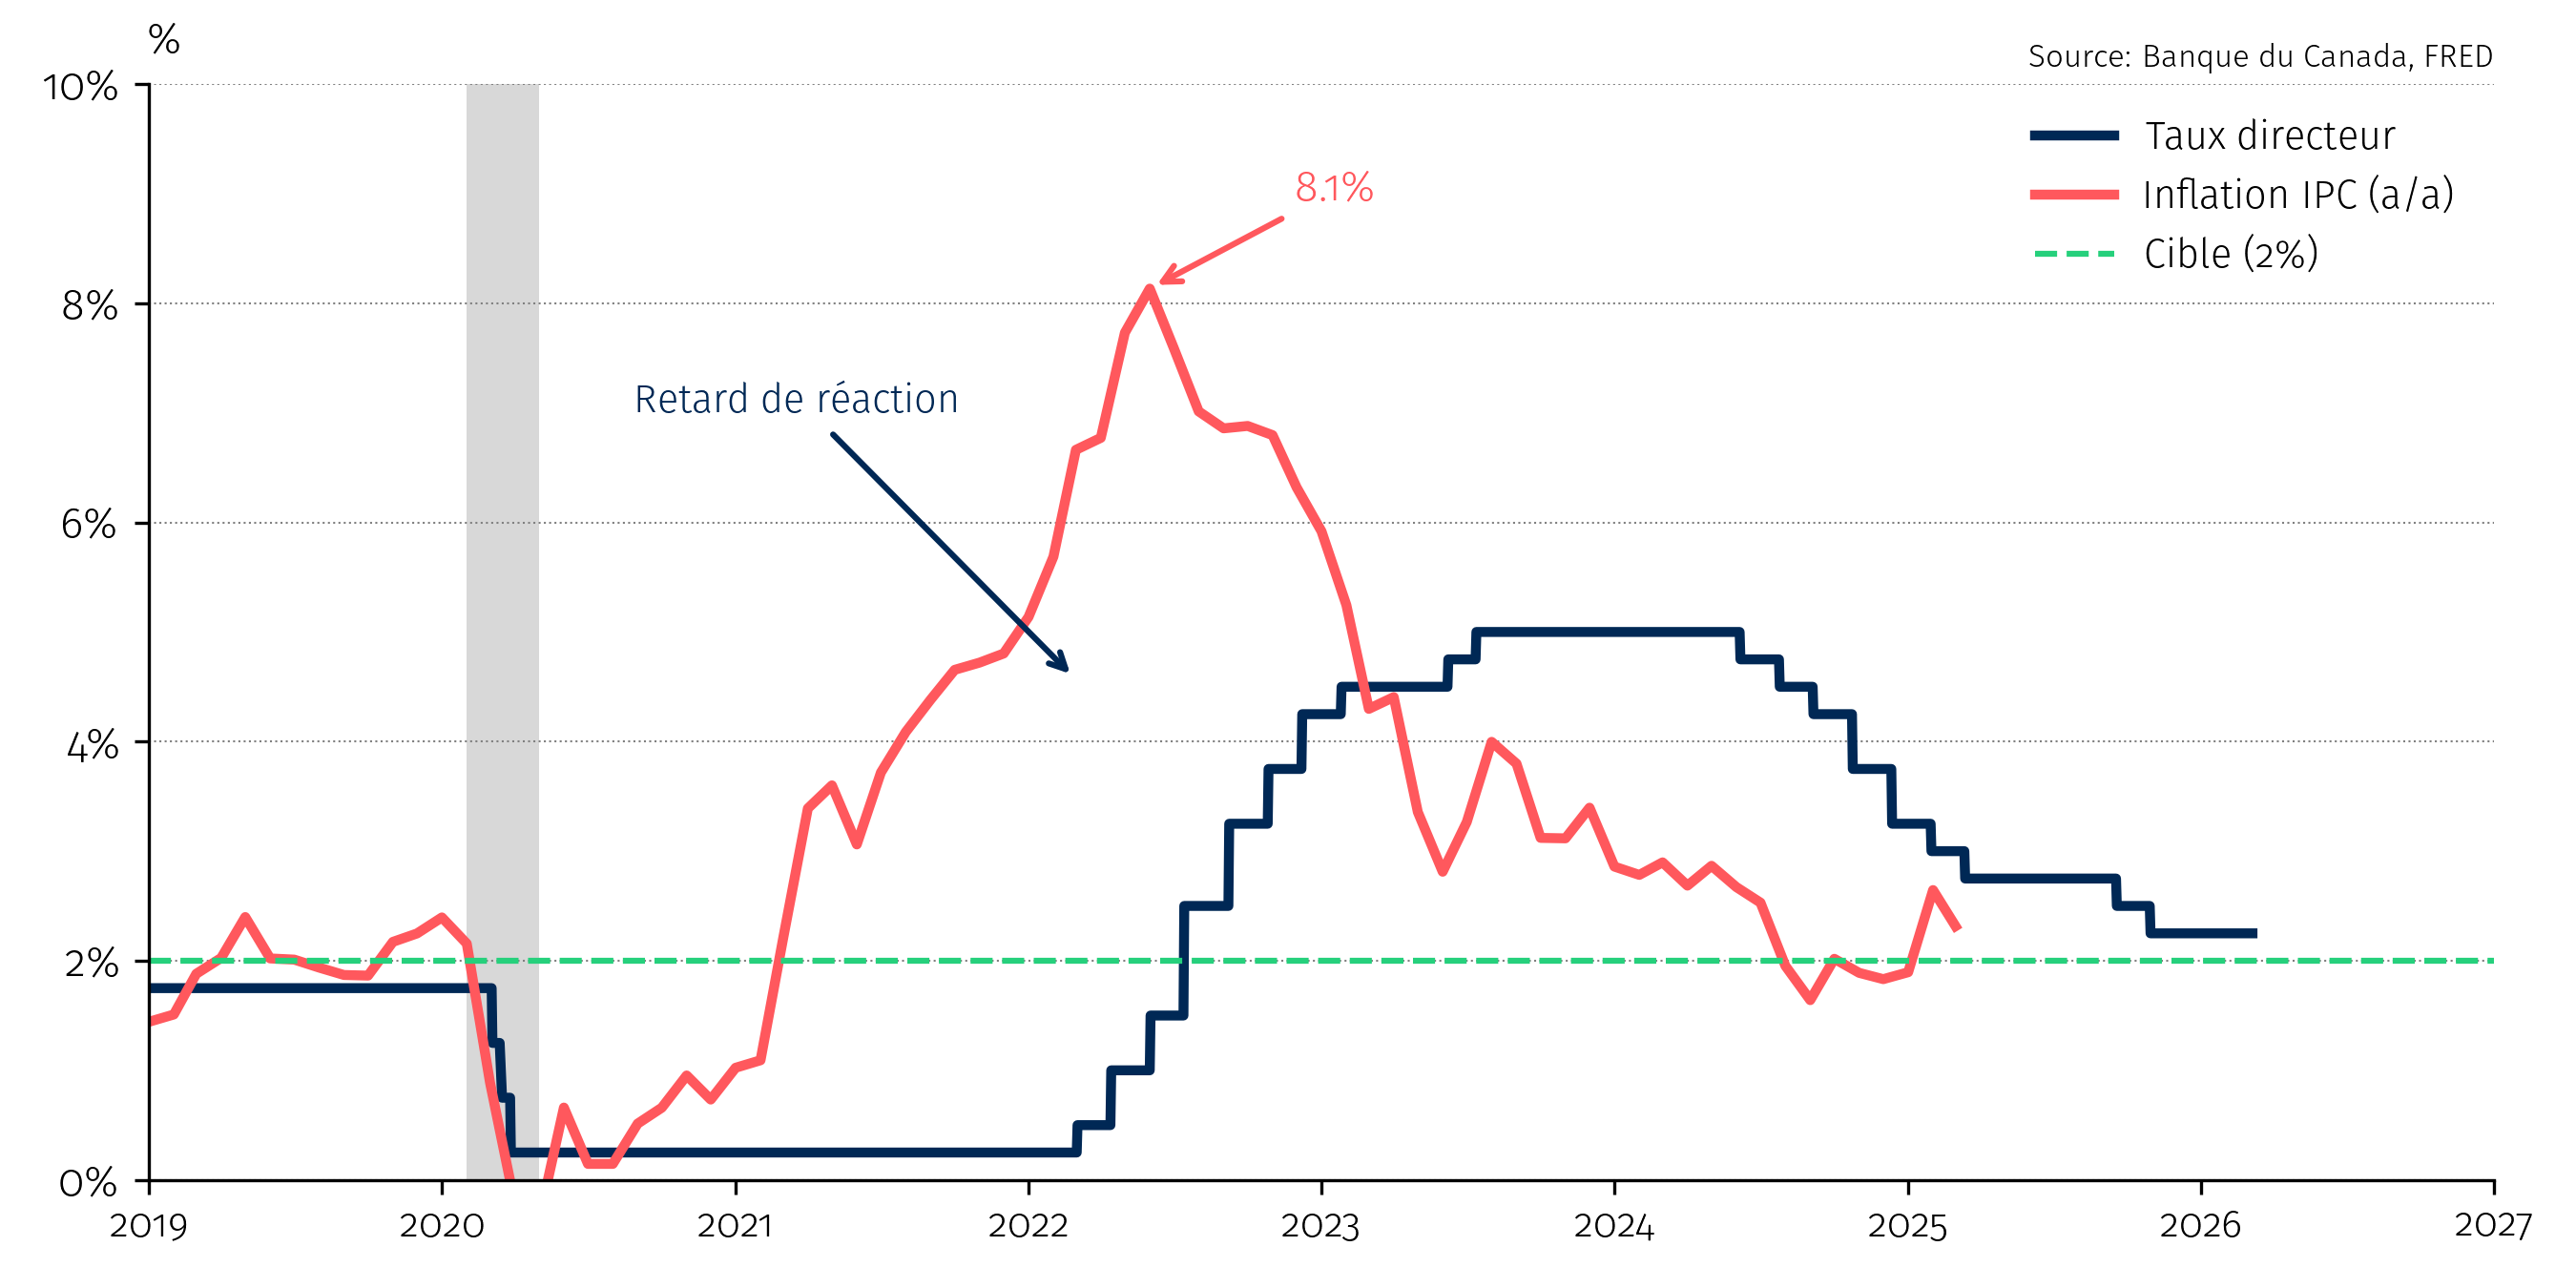
\includegraphics[width=0.95\textwidth, height=0.78\textheight, keepaspectratio]{inflation_vs_rate_2019.png}
   \end{figure}
\end{frame}

\begin{frame}{L'erreur en AD-AS : la relance a d\'{e}pass\'{e} la cible}
   \centering
   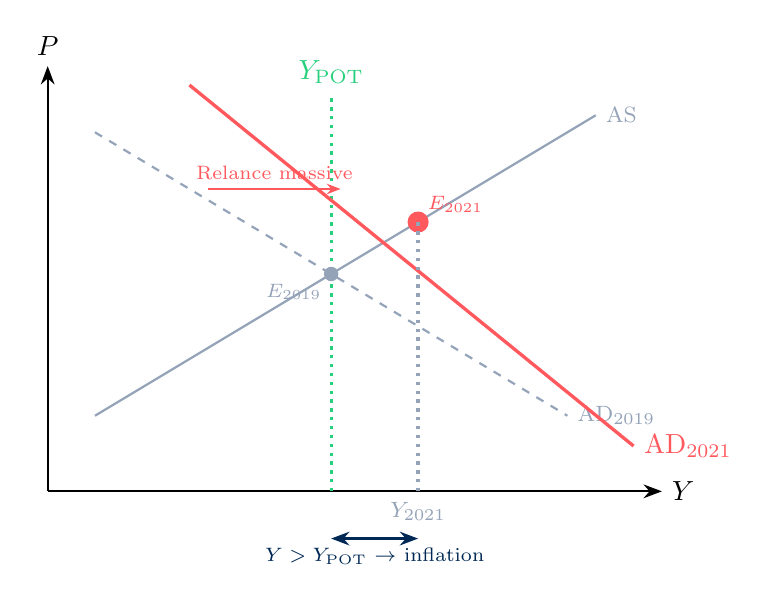
\begin{tikzpicture}[scale=1.2]
      % Axes
      \draw[-{Stealth}, thick] (0,0) -- (6.5,0) node[right] {$Y$};
      \draw[-{Stealth}, thick] (0,0) -- (0,4.5) node[above] {$P$};
      % Y_POT (vertical)
      \draw[HECgreen, very thick, dotted] (3.0,0) -- (3.0,4.2)
         node[above] {$Y_{\text{POT}}$};
      % AS: y = 0.6x + 0.5
      \draw[HECgray, thick] (0.5,0.8) -- (5.8,3.98)
         node[right, font=\footnotesize] {AS};
      % AD original (2019): y = -0.6x + 4.1
      \draw[HECgray, dashed, thick] (0.5,3.8) -- (5.5,0.8)
         node[right, font=\footnotesize] {AD$_{2019}$};
      % AD' shifted far right (massive stimulus): y = -0.6x + 5.2
      \draw[HECcoral, very thick] (1.5,4.3) -- (6.2,0.48)
         node[right] {AD$_{2021}$};
      % Stimulus arrow at y=3.2: AD_2019 at x=1.5, AD_2021 at x=3.33
      \draw[-{Stealth[length=5pt]}, HECcoral, thick] (1.7,3.2) -- (3.1,3.2);
      \node[font=\scriptsize, HECcoral, above] at (2.4,3.2) {Relance massive};
      % Original equilibrium at (3.0, 2.3)
      \filldraw[HECgray] (3.0,2.3) circle (2pt);
      \node[font=\scriptsize, HECgray, below left] at (3.0,2.3) {$E_{2019}$};
      % New equilibrium: -0.6x + 5.2 = 0.6x + 0.5 → 1.2x = 4.7 → x = 3.92, y = 2.85
      \filldraw[HECcoral] (3.92,2.85) circle (3pt);
      \node[font=\scriptsize, HECcoral, above right] at (3.92,2.85) {$E_{2021}$};
      \draw[dotted, very thick, HECgray] (3.92,0) node[below, font=\footnotesize] {$Y_{2021}$} -- (3.92,2.85);
      % Overshoot annotation
      \draw[{Stealth}-{Stealth}, HECnavy, thick] (3.0,-0.5) -- (3.92,-0.5);
      \node[font=\scriptsize, HECnavy, below] at (3.46,-0.5) {$Y > Y_{\text{POT}}$ $\to$ inflation};
   \end{tikzpicture}
\end{frame}

\begin{frame}[t]{Le resserrement le plus rapide en 40 ans}
   \small
   \vspace{0.2cm}
   \textbf{R\'{e}action des banques centrales face \`{a} l'inflation :}
   \vspace{0.15cm}
   \begin{columns}[T]
      \begin{column}{0.47\textwidth}
         \textbf{Banque du Canada :}
         \begin{itemize}
            \setlength\itemsep{0.1cm}
            \item Mars 2022 : premi\`{e}re hausse
            \item Juil.\ 2022 : hausse \guillemotleft~jumbo~\guillemotright\ de \textbf{100 pb}
            \item Juil.\ 2023 : pic \`{a} \textbf{5.00\,\%}
            \item De 0.25\,\% \`{a} 5\,\% en 16 mois
         \end{itemize}
      \end{column}
      \begin{column}{0.47\textwidth}
         \textbf{Fed (r\'{e}serve f\'{e}d\'{e}rale) :}
         \begin{itemize}
            \setlength\itemsep{0.1cm}
            \item Mars 2022 : premi\`{e}re hausse
            \item De 0--0.25\,\% \`{a} \textbf{5.25--5.50\,\%}
            \item 11 hausses en 16 mois
            \item Plus agressif depuis Volcker (1981)
         \end{itemize}
      \end{column}
   \end{columns}
   \vspace{0.15cm}
   \begin{warning}
      Les d\'{e}lais expliquent l'erreur : quand l'inflation a d\'{e}coll\'{e} (mi-2021), les effets complets de la relance de 2020 n'\'{e}taient pas encore visibles. Quand les hausses de taux ont commenc\'{e}, il \'{e}tait d\'{e}j\`{a} tard.
   \end{warning}
\end{frame}

\begin{frame}[t]{D\'{e}fi 3 : cr\'{e}dibilit\'{e} et anticipations}
   \small
   \vspace{0.2cm}
   \textbf{Les anticipations d'inflation sont auto-r\'{e}alisatrices :}
   \vspace{0.15cm}
   \begin{itemize}
      \setlength\itemsep{0.15cm}
      \item Si les agents \textbf{croient} que l'inflation sera \'{e}lev\'{e}e $\to$ ils demandent des hausses salariales $\to$ co\^{u}ts $\uparrow$ $\to$ prix $\uparrow$ $\to$ l'inflation \textbf{augmente r\'{e}ellement}
      \item Si la BdC est \textbf{cr\'{e}dible}, les anticipations restent \guillemotleft~ancr\'{e}es~\guillemotright\ \`{a} 2\,\%
      \item Quand la cr\'{e}dibilit\'{e} est perdue, combattre l'inflation devient \textbf{beaucoup plus co\^{u}teux} (ex.\ : Volcker 1981, taux \`{a} 20\,\%, r\'{e}cession majeure)
   \end{itemize}
   \vspace{0.15cm}
   \begin{warning}
      L'ind\'{e}pendance de la banque centrale n'est pas un luxe acad\'{e}mique --- c'est le fondement de sa cr\'{e}dibilit\'{e}. Quand un gouvernement menace cette ind\'{e}pendance, les march\'{e}s r\'{e}agissent imm\'{e}diatement.
   \end{warning}
\end{frame}

\begin{frame}[t]{La courbe de Phillips}
   \small
   \vspace{0.05cm}
   \begin{columns}[c]
      \begin{column}{0.52\textwidth}
         \centering
         {\small\textbf{\textcolor{HECcoral}{Court terme}}}
         \par\smallskip
         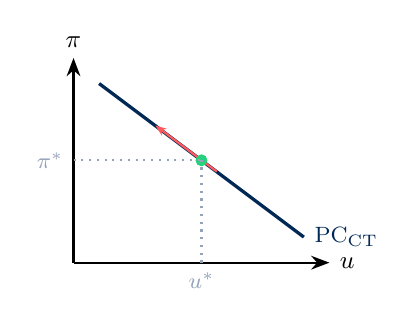
\begin{tikzpicture}[scale=0.65]
            \draw[-{Stealth}, thick] (0,0) -- (5,0) node[right, font=\small] {$u$};
            \draw[-{Stealth}, thick] (0,0) -- (0,4) node[above, font=\small] {$\pi$};
            % SR Phillips curve
            \draw[HECnavy, very thick] (0.5,3.5) -- (4.5,0.5)
               node[right, font=\footnotesize] {PC$_{\text{CT}}$};
            % Tradeoff arrow along SR curve (NW direction)
            \draw[-{Stealth[length=4pt]}, HECcoral, thick] (2.8,1.78) -- (1.6,2.68);
            % Equilibrium dot
            \filldraw[HECgreen] (2.5,2.0) circle (3pt);
            % Dotted lines
            \draw[dotted, thick, HECgray] (2.5,0) node[below, font=\footnotesize] {$u^*$} -- (2.5,2.0);
            \draw[dotted, thick, HECgray] (0,2.0) node[left, font=\footnotesize] {$\pi^*$} -- (2.5,2.0);
         \end{tikzpicture}
         \par\smallskip
         {\footnotesize Arbitrage $u \leftrightarrow \pi$}
      \end{column}
      \begin{column}{0.52\textwidth}
         \centering
         {\small\textbf{\textcolor{HECnavy}{Long terme}}}
         \par\smallskip
         \begin{tikzpicture}[scale=0.65]
            \draw[-{Stealth}, thick] (0,0) -- (5,0) node[right, font=\small] {$u$};
            \draw[-{Stealth}, thick] (0,0) -- (0,4) node[above, font=\small] {$\pi$};
            % LR Phillips curve (vertical)
            \draw[HECgreen, ultra thick, dotted] (2.5,0.3) -- (2.5,3.8)
               node[above, font=\footnotesize] {PC$_{\text{LT}}$};
            \node[font=\footnotesize, HECgray, below] at (2.5,0) {$u^*$};
         \end{tikzpicture}
         \par\smallskip
         {\footnotesize Pas d'arbitrage permanent}
      \end{column}
   \end{columns}
   \vspace{0.05cm}
   \begin{keyinsight}
      \`{A} long terme, la courbe de Phillips est \textbf{verticale} : on ne peut pas \guillemotleft~acheter~\guillemotright\ un ch\^{o}mage durablement plus bas en tol\'{e}rant plus d'inflation.
   \end{keyinsight}
\end{frame}

\begin{frame}[t]{L'atterrissage en douceur}
   \framesubtitle{L'art de ralentir sans provoquer une r\'{e}cession}
   \small
   \vspace{0.2cm}
   \textbf{2023--2025 : un relatif succ\`{e}s\,?}
   \vspace{0.15cm}
   \begin{itemize}
      \setlength\itemsep{0.15cm}
      \item Inflation ramen\'{e}e de 8\,\% \`{a} $\sim$2\,\% au Canada
      \item Hausse du ch\^{o}mage \textbf{mod\'{e}r\'{e}e} (pas de r\'{e}cession technique)
      \item \'{E}quilibre d\'{e}licat entre \guillemotleft~trop~\guillemotright\ et \guillemotleft~pas assez~\guillemotright
   \end{itemize}
   \vspace{0.15cm}
   \textbf{Historiquement, c'est l'exception :}
   \vspace{0.1cm}
   \begin{itemize}
      \setlength\itemsep{0.1cm}
      \item 1981 : Volcker tue l'inflation mais provoque une r\'{e}cession majeure
      \item 1994 : Greenspan r\'{e}ussit un atterrissage en douceur (rare)
      \item 2022--25 : la plupart des pays ont \'{e}vit\'{e} la r\'{e}cession (pour l'instant)
   \end{itemize}
\end{frame}

\begin{frame}[t]{La r\`{e}gle de Taylor (intuition)}
   \small
   \vspace{0.05cm}
   \begin{defbox}[R\`{e}gle de Taylor]
      La banque centrale r\'{e}agit syst\'{e}matiquement \`{a} \textbf{deux} variables : l'\'{e}cart d'inflation et l'\'{e}cart de production.
   \end{defbox}
   \vspace{0.05cm}
   \footnotesize
   \begin{itemize}
      \setlength\itemsep{0.08cm}
      \item Si $\pi > 2\,\%$ : \textbf{monter} le taux (plus que l'\'{e}cart d'inflation)
      \item Si $Y < Y_{\text{POT}}$ : \textbf{baisser} le taux pour stimuler l'activit\'{e}
      \item Cadre \textbf{disciplin\'{e}} vs.\ simple jugement discr\'{e}tionnaire
   \end{itemize}
   \vspace{0.05cm}
   \small
   \begin{keyinsight}[Principe de Taylor]
      Quand l'inflation monte de 1 point, le taux directeur doit monter de \textbf{plus} d'un point. Sinon, le taux r\'{e}el baisse et la politique devient involontairement expansionniste.
   \end{keyinsight}
\end{frame}

\begin{frame}[t]{La borne z\'{e}ro : quand l'outil conventionnel ne suffit plus}
   \small
   \vspace{0.2cm}
   \textbf{Probl\`{e}me :} le taux directeur ne peut pas descendre beaucoup en dessous de 0\,\%.
   \vspace{0.2cm}
   \begin{itemize}
      \setlength\itemsep{0.2cm}
      \item En 2009 et 2020, la BdC et la Fed ont atteint $\sim$0\,\%
      \item L'\'{e}conomie avait encore besoin de stimulation $\to$ \guillemotleft~pousser sur une corde~\guillemotright
      \item Solution : outils \textbf{non conventionnels} (section suivante)
   \end{itemize}
   \vspace{0.1cm}
   \begin{figure}
      \centering
      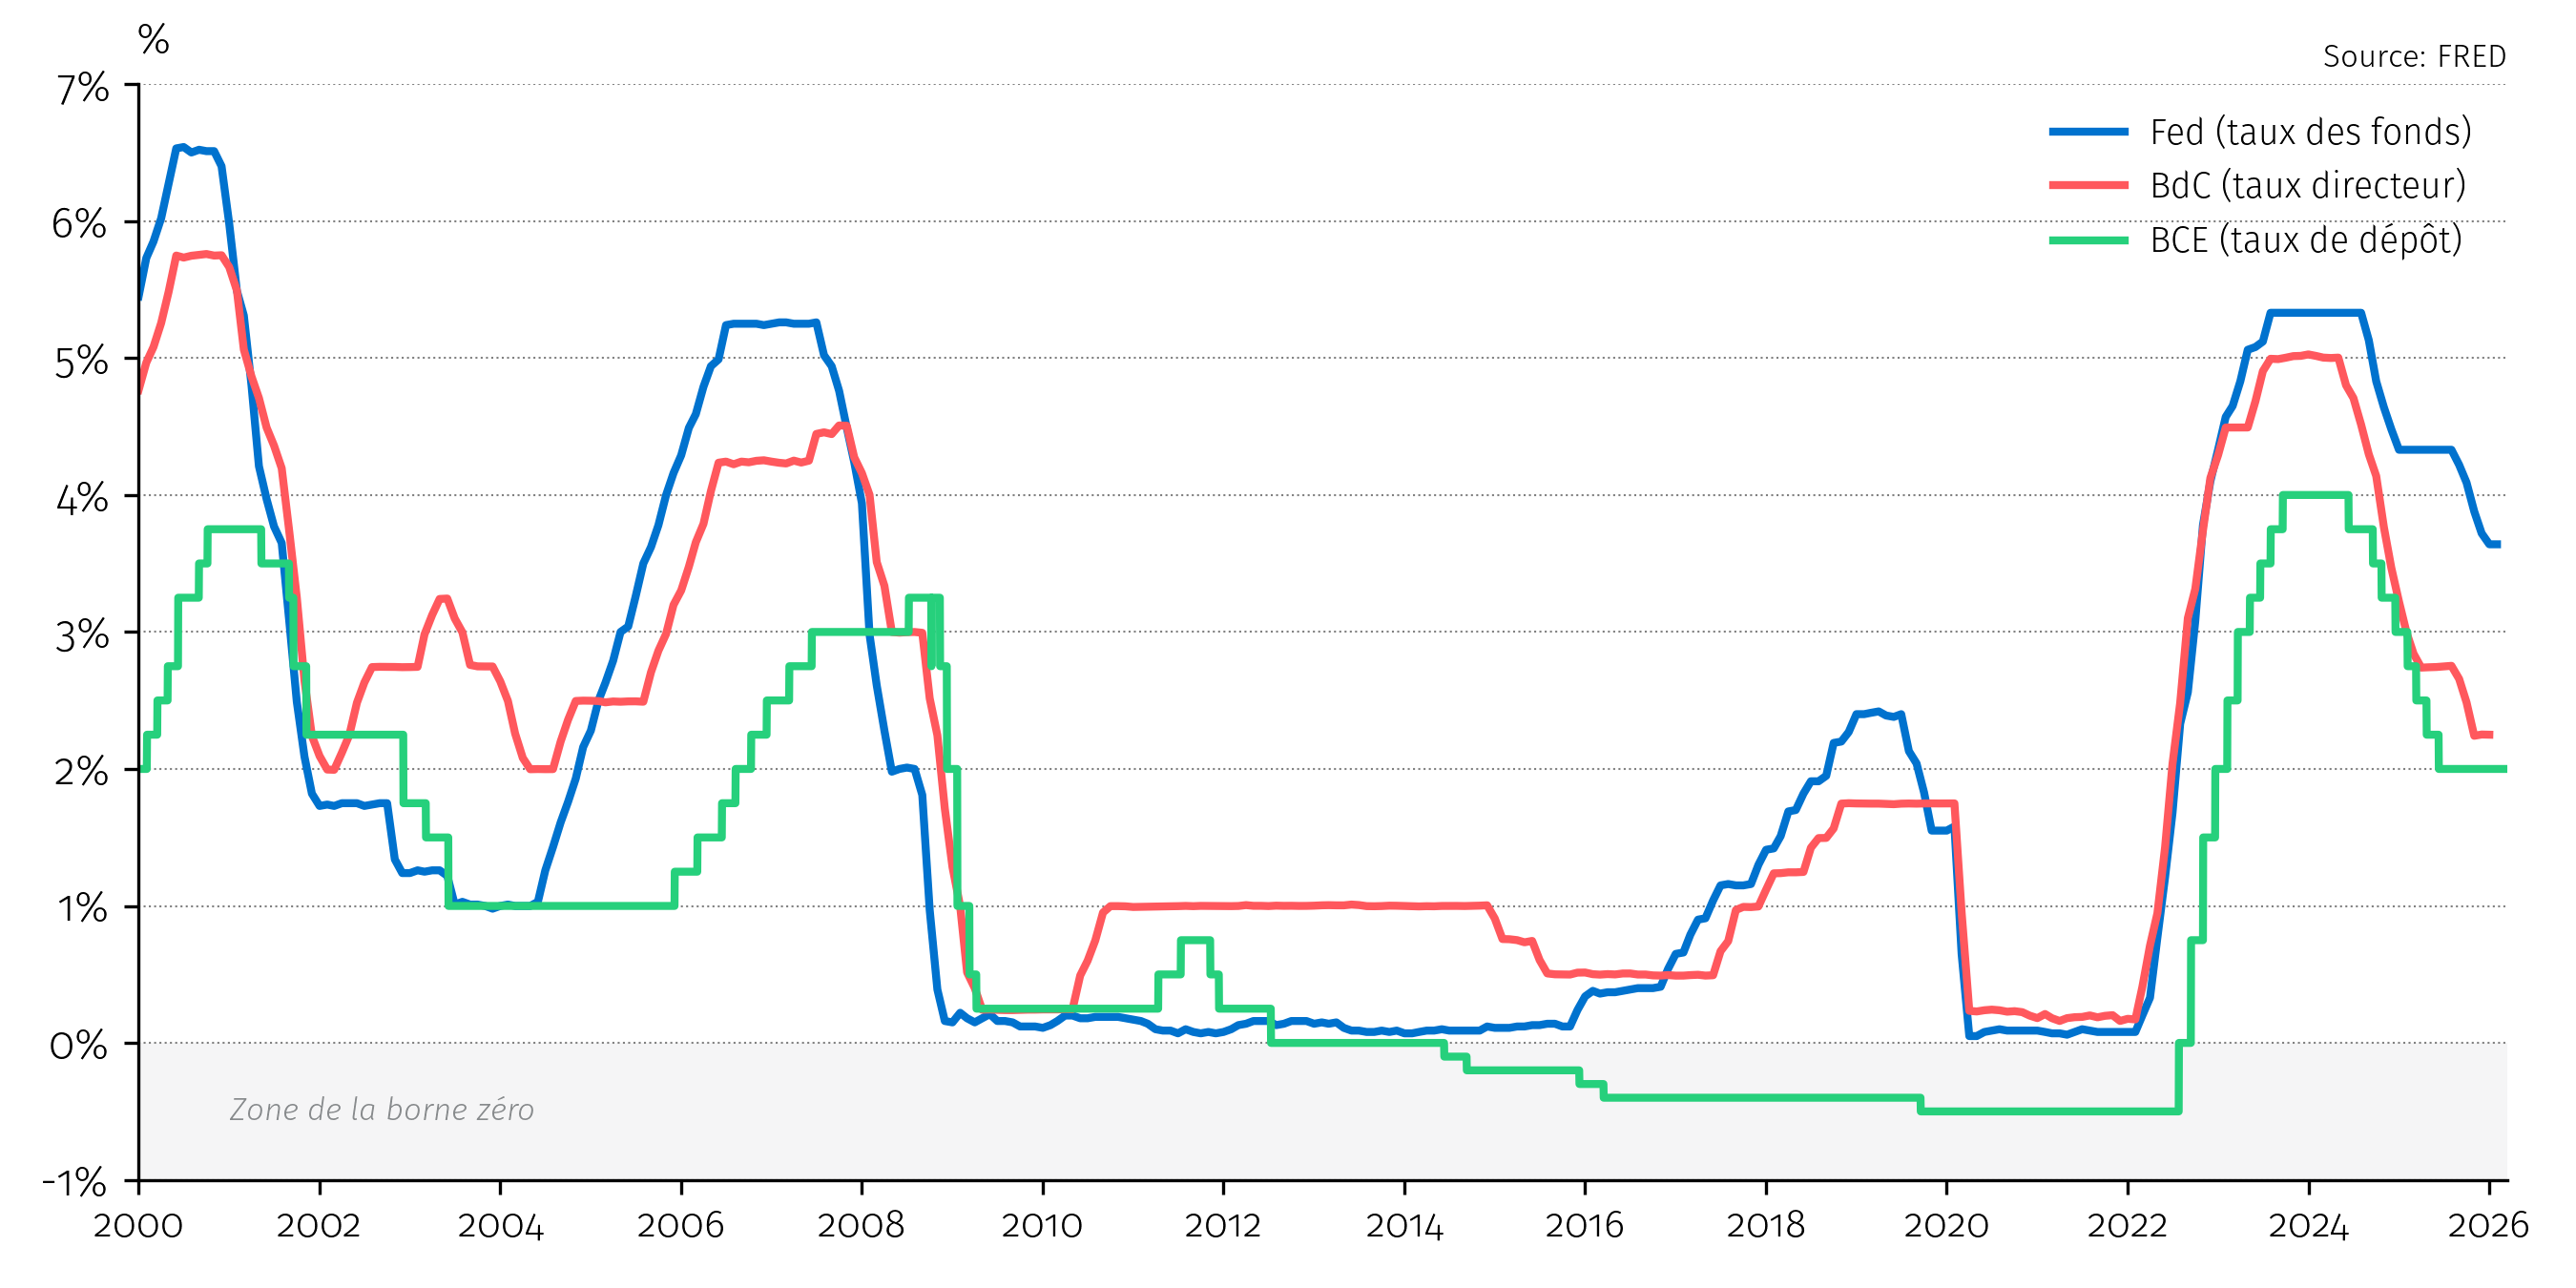
\includegraphics[width=0.80\textwidth, height=0.35\textheight, keepaspectratio]{policy_rates_global.png}
   \end{figure}
\end{frame}

\begin{frame}{Exercice en classe}
   \begin{exercise}
      La BdC \textbf{baisse} le taux directeur de 50 points de base en r\'{e}ponse \`{a} une contraction \'{e}conomique.
      \\[6pt]
      \textbf{Questions :}
      \begin{enumerate}
         \setlength\itemsep{0.1cm}
         \item Montrez l'effet sur un diagramme AD-AS.
         \item Quel est l'effet attendu sur $Y$, $P$ et le ch\^{o}mage\,?
         \item Pourquoi l'effet complet ne se fera-t-il sentir que dans 18 mois\,?
      \end{enumerate}
   \end{exercise}
\end{frame}

% ============================================================================

\begin{frame}{Plan}
   \begin{enumerate}
      \setlength\itemsep{0.5cm}
      \item {\color{gray!50}Pourquoi combattre les r\'{e}cessions\,?}
      \item {\color{gray!50}La politique mon\'{e}taire conventionnelle}
      \item {\color{gray!50}D\'{e}fis et limites de la politique mon\'{e}taire}
      \item \textbf{La politique mon\'{e}taire non conventionnelle}
      \item La politique budg\'{e}taire
      \item La dette publique
   \end{enumerate}
\end{frame}

% ============================================================================
\sectionframe{La politique mon\'{e}taire non conventionnelle}
% ============================================================================

\begin{frame}[t]{Quand la bo\^{i}te \`{a} outils conventionnelle est vide}
   \vspace{0.3cm}
   \textbf{Trois outils non conventionnels :}
   \vspace{0.3cm}
   \begin{columns}[T,onlytextwidth]
      \begin{column}{0.30\textwidth}
         \begin{tcolorbox}[colback=HECgreen!8, colframe=HECgreen, boxrule=0.5pt, arc=8pt,
            top=4pt, bottom=4pt, left=6pt, right=6pt]
            \centering\footnotesize\textbf{Indications prospectives}\\(\textit{forward guidance})\\[3pt]
            Communiquer ses intentions futures pour influencer les anticipations
         \end{tcolorbox}
      \end{column}
      \begin{column}{0.30\textwidth}
         \begin{tcolorbox}[colback=HECnavy!8, colframe=HECnavy, boxrule=0.5pt, arc=8pt,
            top=4pt, bottom=4pt, left=6pt, right=6pt]
            \centering\footnotesize\textbf{Assouplissement quantitatif}\\(\textit{quantitative easing})\\[3pt]
            Acheter des obligations pour injecter des liquidit\'{e}s
         \end{tcolorbox}
      \end{column}
      \begin{column}{0.30\textwidth}
         \begin{tcolorbox}[colback=HECcoral!8, colframe=HECcoral, boxrule=0.5pt, arc=8pt,
            top=4pt, bottom=4pt, left=6pt, right=6pt]
            \centering\footnotesize\textbf{Taux n\'{e}gatifs}\\[3pt]
            Exp\'{e}riment\'{e}s par la BCE et la BoJ pour forcer les banques \`{a} pr\^{e}ter
         \end{tcolorbox}
      \end{column}
   \end{columns}
\end{frame}

\begin{frame}[t]{Indications prospectives (\textit{forward guidance})}
   \small
   \vspace{0.2cm}
   \textbf{Id\'{e}e :} la banque centrale s'engage publiquement \`{a} garder les taux bas \guillemotleft~aussi longtemps que n\'{e}cessaire~\guillemotright.
   \vspace{0.2cm}
   \begin{itemize}
      \setlength\itemsep{0.2cm}
      \item M\^{e}me si le taux \`{a} un jour est d\'{e}j\`{a} \`{a} 0\,\%, les taux \textbf{longs} d\'{e}pendent des \textbf{anticipations} du taux futur
      \item En s'engageant \`{a} garder les taux bas $\to$ taux longs $\downarrow$ $\to$ stimulation de $C$ et $I$
      \item Exemple : le \textit{dot plot} de la Fed (projections des membres du FOMC)
   \end{itemize}
   \vspace{0.15cm}
   \begin{keyinsight}
      La communication est devenue un \textbf{outil de politique mon\'{e}taire} \`{a} part enti\`{e}re. Ce que la BdC \textit{dit} peut \^{e}tre aussi important que ce qu'elle \textit{fait}.
   \end{keyinsight}
\end{frame}

\begin{frame}[t]{Assouplissement quantitatif (QE)}
   \small
   \vspace{0.2cm}
   \begin{defbox}[Assouplissement quantitatif]
      La banque centrale ach\`{e}te massivement des \textbf{obligations gouvernementales} (et parfois corporatives) sur les march\'{e}s secondaires.
   \end{defbox}
   \vspace{0.1cm}
   \textbf{M\'{e}canisme :}
   \vspace{0.05cm}
   \begin{enumerate}
      \setlength\itemsep{0.1cm}
      \item BdC ach\`{e}te des obligations $\to$ prix des obligations $\uparrow$
      \item Prix des obligations $\uparrow$ $\to$ taux de rendement (long terme) $\downarrow$
      \item Taux long terme $\downarrow$ $\to$ stimule l'emprunt et l'investissement
      \item Liquidit\'{e}s inject\'{e}es $\to$ banques ont plus de fonds \`{a} pr\^{e}ter
   \end{enumerate}
   \vspace{0.1cm}
   \textbf{Utilis\'{e} en :} 2008--14 (Fed, BCE), 2020--22 (Fed, BdC, BCE)
\end{frame}

\begin{frame}{Le bilan de la BdC : le QE en images}
   \begin{figure}
      \centering
      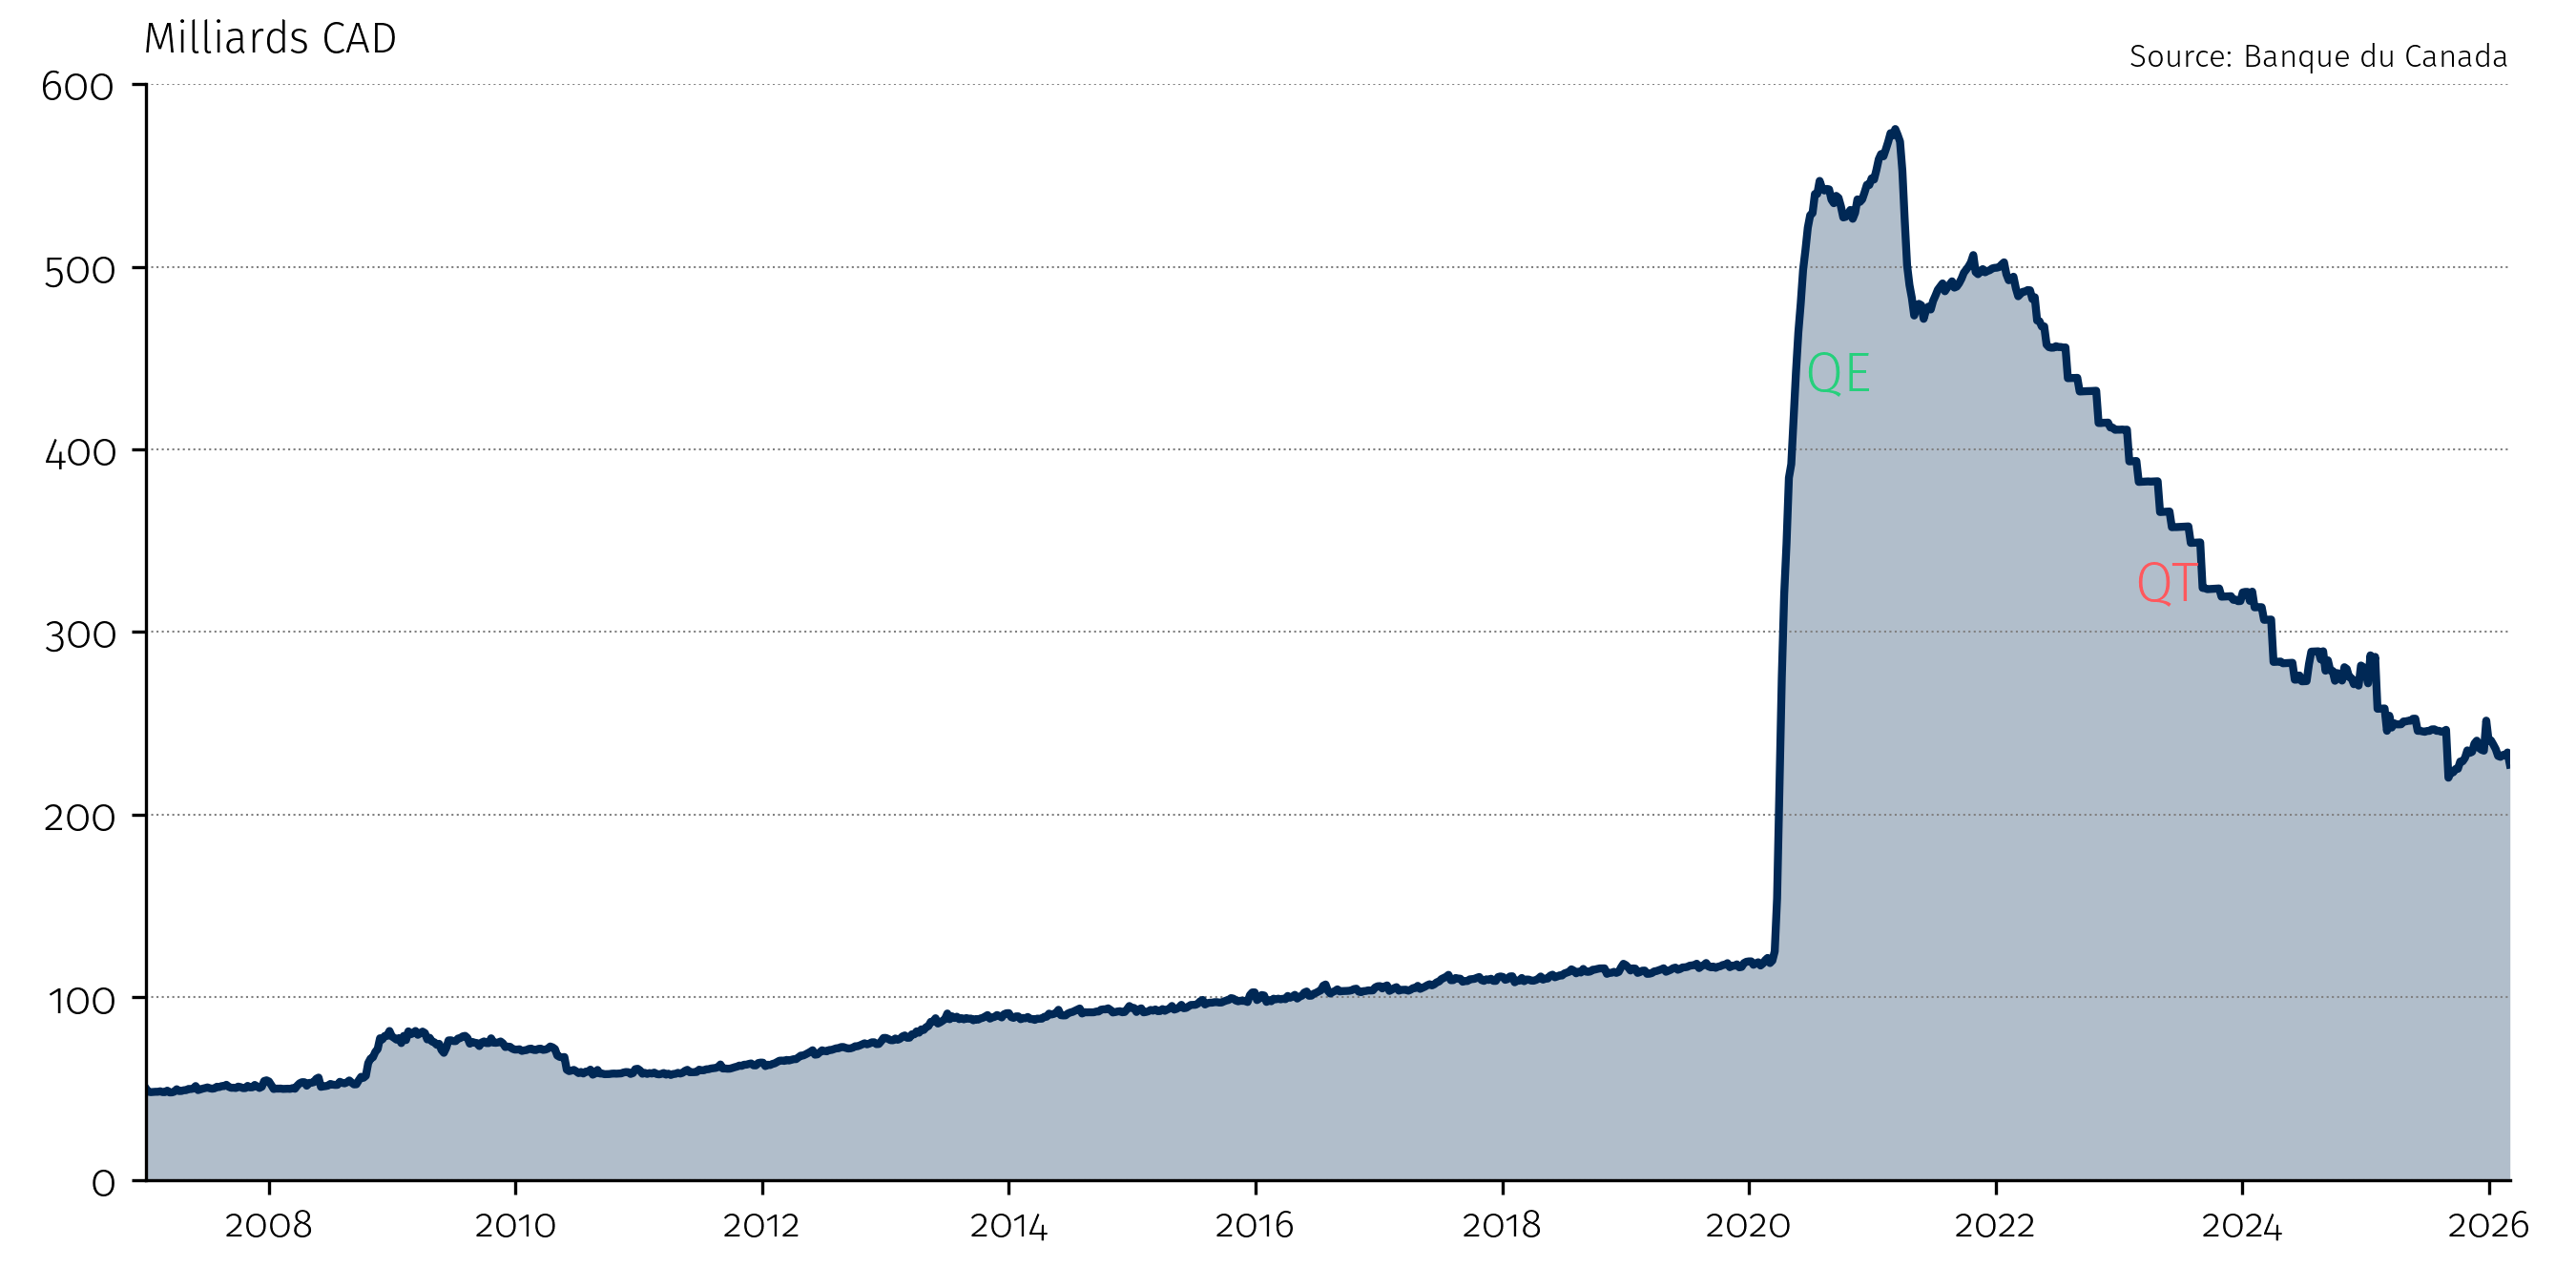
\includegraphics[width=0.95\textwidth, height=0.78\textheight, keepaspectratio]{boc_balance_sheet.png}
   \end{figure}
\end{frame}

\begin{frame}[t]{QE : succ\`{e}s et risques}
   \small
   \vspace{0.2cm}
   \begin{columns}[T]
      \begin{column}{0.47\textwidth}
         \textbf{\textcolor{HECgreen}{B\'{e}n\'{e}fices :}}
         \begin{itemize}
            \setlength\itemsep{0.15cm}
            \item $\downarrow$ taux longs, m\^{e}me quand le taux court est \`{a} z\'{e}ro
            \item $\uparrow$ prix des actifs $\to$ effet de richesse
            \item A \'{e}vit\'{e} une d\'{e}pression en 2008--09 et 2020
         \end{itemize}
      \end{column}
      \begin{column}{0.47\textwidth}
         \textbf{\textcolor{HECcoral}{Risques :}}
         \begin{itemize}
            \setlength\itemsep{0.15cm}
            \item $\uparrow$ in\'{e}galit\'{e}s : les d\'{e}tenteurs d'actifs profitent davantage
            \item Risque de \textbf{bulles} sp\'{e}culatives
            \item Inflation retard\'{e}e (2021--22\,?)
            \item \textbf{Resserrement quantitatif} (QT) difficile
         \end{itemize}
      \end{column}
   \end{columns}
   \vspace{0.2cm}
   \begin{keyinsight}
      Le QE a montr\'{e} que les banques centrales ne sont jamais vraiment \`{a} court de munitions --- mais chaque nouvel outil a des \textbf{effets secondaires croissants}.
   \end{keyinsight}
\end{frame}

% ============================================================================

\begin{frame}{Plan}
   \begin{enumerate}
      \setlength\itemsep{0.5cm}
      \item {\color{gray!50}Pourquoi combattre les r\'{e}cessions\,?}
      \item {\color{gray!50}La politique mon\'{e}taire conventionnelle}
      \item {\color{gray!50}D\'{e}fis et limites de la politique mon\'{e}taire}
      \item {\color{gray!50}La politique mon\'{e}taire non conventionnelle}
      \item \textbf{La politique budg\'{e}taire}
      \item La dette publique
   \end{enumerate}
\end{frame}

% ============================================================================
\sectionframe{La politique budg\'{e}taire}
% ============================================================================

\begin{frame}[t]{L'autre levier : le gouvernement}
   \small
   \vspace{0.2cm}
   \textbf{Trois canaux pour stimuler AD :}
   \vspace{0.2cm}
   \begin{enumerate}
      \setlength\itemsep{0.2cm}
      \item \textbf{D\'{e}penses publiques ($G \uparrow$)} --- effet direct sur le PIB (infrastructure, d\'{e}fense, sant\'{e})
      \item \textbf{Transferts aux m\'{e}nages} --- effet indirect via $C$ (ch\`{e}ques, assurance-emploi)
      \item \textbf{Baisses d'imp\^{o}ts ($T \downarrow$)} --- effet indirect via $C$ et $I$ (revenu disponible $\uparrow$)
   \end{enumerate}
   \vspace{0.2cm}
   \begin{keyinsight}[Diff\'{e}rence fondamentale]
      $G$ entre \textbf{directement} dans le PIB ($Y = C + I + G + NX$). Les transferts et baisses d'imp\^{o}ts ne stimulent le PIB que si les m\'{e}nages \textbf{d\'{e}pensent} l'argent re\c{c}u.
   \end{keyinsight}
\end{frame}

\begin{frame}[t]{L'effet multiplicateur}
   \small
   \vspace{0.05cm}
   \begin{defbox}[Le multiplicateur]
      Un dollar d\'{e}pens\'{e} par le gouvernement g\'{e}n\`{e}re \textbf{plus} d'un dollar de PIB gr\^{a}ce \`{a} la propagation dans l'\'{e}conomie.
   \end{defbox}
   \vspace{0.02cm}
   \footnotesize
   \begin{tcolorbox}[
      colback=white, colframe=HECnavy, colbacktitle=HECnavy,
      title=\textbf{Exemple simplifi\'{e}}, fonttitle=\footnotesize, boxrule=0.5pt, arc=8pt,
      top=2pt, bottom=2pt, left=6pt, right=6pt]
      Suppos\'{e} : propension marginale \`{a} consommer = 0.8 (80\,\% du revenu est d\'{e}pens\'{e}).
      \vspace{0.02cm}

      \renewcommand{\arraystretch}{1.0}
      \centering
      \begin{tabularx}{0.85\linewidth}{X r}
         \rowcolor{HECnavy!10}
         \textbf{Ronde} & \textbf{D\'{e}pense suppl.} \\
         \hline
         1.\ Gouvernement d\'{e}pense & 100\,M\$ \\
         2.\ R\'{e}cipiendaires d\'{e}pensent 80\,\% & 80\,M\$ \\
         3.\ La vague suivante & 64\,M\$ \\
         \ldots & \ldots \\
         \hline
         \textbf{Total} & $\frac{100}{1-0.8}$ = \textbf{500\,M\$}
      \end{tabularx}
   \end{tcolorbox}
   \vspace{0.02cm}
   {\footnotesize Multiplicateur = $\frac{1}{1 - \text{PMC}} = \frac{1}{0.2} = 5$ (cas extr\^{e}me sans fuites).}
\end{frame}

\begin{frame}[t]{Le d\'{e}bat sur le multiplicateur}
   \small
   \vspace{0.2cm}
   \textbf{Le multiplicateur est-il vraiment sup\'{e}rieur \`{a} 1\,?}
   \vspace{0.2cm}
   \begin{itemize}
      \setlength\itemsep{0.2cm}
      \item \textbf{Effet d'\'{e}viction} (\textit{crowding out}) : $G \uparrow$ $\to$ emprunt public $\uparrow$ $\to$ taux d'int\'{e}r\^{e}t $\uparrow$ $\to$ $I$ priv\'{e} $\downarrow$
      \item L'\'{e}viction \textbf{r\'{e}duit} le multiplicateur (parfois \`{a} moins de 1)
      \item \textbf{\'{E}vidence empirique :} le multiplicateur est plus grand en r\'{e}cession (quand les ressources sont inutilis\'{e}es, pas d'\'{e}viction) et plus petit en expansion
   \end{itemize}
   \vspace{0.15cm}
   \begin{warning}
      Un plan de relance en p\'{e}riode de \textbf{plein emploi} risque surtout de g\'{e}n\'{e}rer de l'inflation et d'\'{e}vincer l'investissement priv\'{e}, avec peu de gain sur le PIB r\'{e}el.
   \end{warning}
\end{frame}

\begin{frame}{Expansion budg\'{e}taire dans le mod\`{e}le AD-AS}
   \centering
   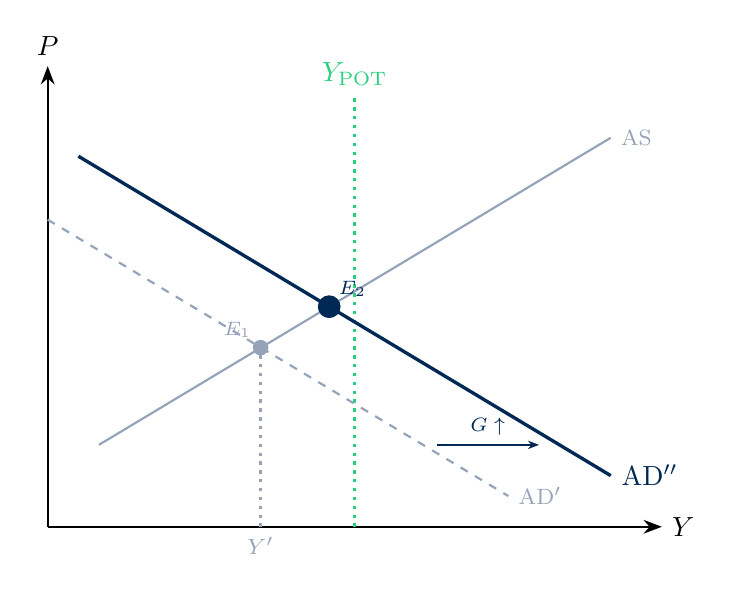
\begin{tikzpicture}[scale=1.3]
      % Axes
      \draw[-{Stealth}, thick] (0,0) -- (6,0) node[right] {$Y$};
      \draw[-{Stealth}, thick] (0,0) -- (0,4.5) node[above] {$P$};
      % Y_POT (vertical)
      \draw[HECgreen, very thick, dotted] (3.0,0) -- (3.0,4.2)
         node[above] {$Y_{\text{POT}}$};
      % AS: y = 0.6x + 0.5
      \draw[HECgray, thick] (0.5,0.8) -- (5.5,3.8)
         node[right, font=\footnotesize] {AS};
      % AD' (recession): y = -0.6x + 3.0
      \draw[HECgray, dashed, thick] (0.0,3.0) -- (4.5,0.3)
         node[right, font=\footnotesize] {AD$'$};
      % AD'' (after fiscal): y = -0.6x + 3.8
      \draw[HECnavy, very thick] (0.3,3.62) -- (5.5,0.5)
         node[right] {AD$''$};
      % Fiscal policy arrow at y=0.8: AD' at x=3.67, AD'' at x=5.0
      \draw[-{Stealth[length=4pt]}, HECnavy, thick] (3.8,0.8) -- (4.8,0.8);
      \node[font=\scriptsize, HECnavy, above] at (4.3,0.8) {$G \uparrow$};
      % Recession equilibrium
      \filldraw[HECgray] (2.08,1.75) circle (2pt);
      \node[font=\scriptsize, HECgray, above left] at (2.08,1.75) {$E_1$};
      % New equilibrium
      \filldraw[HECnavy] (2.75,2.15) circle (3pt);
      \node[font=\scriptsize, HECnavy, above right] at (2.75,2.15) {$E_2$};
      \draw[dotted, very thick, HECgray] (2.08,0) node[below, font=\footnotesize] {$Y'$} -- (2.08,1.75);
   \end{tikzpicture}
\end{frame}

\begin{frame}[t]{Application : la PCU en 2020}
   \small
   \vspace{0.1cm}
   \textbf{Prestation canadienne d'urgence (PCU/CERB) :}
   \vspace{0.1cm}
   \begin{itemize}
      \setlength\itemsep{0.1cm}
      \item 2\,000\,\$ par mois pour les travailleurs affect\'{e}s par la pand\'{e}mie
      \item Co\^{u}t total : $\sim$82 milliards \$
      \item 8.9 millions de demandeurs (dans un pays de 38 millions)
   \end{itemize}
   \vspace{0.1cm}
   \textbf{Effet :}
   \vspace{0.05cm}
   \begin{itemize}
      \setlength\itemsep{0.05cm}
      \item A \textbf{stabilis\'{e} le revenu} des m\'{e}nages $\to$ \'{e}vit\'{e} un effondrement de $C$
      \item Mais : a contribu\'{e} \`{a} l'\textbf{exc\`{e}s de demande} en 2021--22 $\to$ inflation
   \end{itemize}
   \vspace{0.05cm}
   \begin{bizimplication}
      Les transferts d'urgence sont un pare-feu efficace \`{a} court terme. Le d\'{e}fi est de savoir \textbf{quand les retirer}.
   \end{bizimplication}
\end{frame}

\begin{frame}[t]{Application : l'\textit{American Rescue Plan} (2021)}
   \small
   \vspace{0.2cm}
   \textbf{Le d\'{e}bat Summers vs.\ Biden :}
   \vspace{0.15cm}
   \begin{itemize}
      \setlength\itemsep{0.15cm}
      \item Plan de relance de \textbf{1\,900 milliards \$} US (mars 2021)
      \item \'{E}cart de production estim\'{e} \`{a} $\sim$700 milliards \$
      \item Larry Summers (Harvard, ex-secr\'{e}taire au Tr\'{e}sor) : \guillemotleft~C'est trop\,! \c{C}a va g\'{e}n\'{e}rer de l'inflation.~\guillemotright
      \item Administration Biden : \guillemotleft~Mieux vaut en faire trop que pas assez.~\guillemotright
   \end{itemize}
   \vspace{0.15cm}
   \textbf{R\'{e}sultat :} les deux avaient partiellement raison.
   \vspace{0.1cm}
   \begin{itemize}
      \setlength\itemsep{0.1cm}
      \item Reprise \'{e}conomique rapide (PIB au-dessus du potentiel d\`{e}s fin 2021)
      \item Mais inflation \`{a} 9\,\% en juin 2022 --- le plus haut niveau en 40 ans
   \end{itemize}
\end{frame}

\begin{frame}[t]{Aust\'{e}rit\'{e} vs.\ relance : le \textit{timing} est tout}
   \small
   \vspace{0.2cm}
   \begin{columns}[T]
      \begin{column}{0.47\textwidth}
         \textbf{\textcolor{HECcoral}{Aust\'{e}rit\'{e} en r\'{e}cession}}\\[4pt]
         {\footnotesize
         Gr\`{e}ce, 2010--2015 :
         \begin{itemize}
            \setlength\itemsep{0.1cm}
            \item Coupes budg\'{e}taires de 30\,\%
            \item PIB chute de 25\,\%
            \item Ch\^{o}mage atteint 27\,\%
         \end{itemize}
         $\to$ L'aust\'{e}rit\'{e} a \textbf{aggrav\'{e}} la crise}
      \end{column}
      \begin{column}{0.47\textwidth}
         \textbf{\textcolor{HECgreen}{Relance bien calibr\'{e}e}}\\[4pt]
         {\footnotesize
         Canada, 2020 :
         \begin{itemize}
            \setlength\itemsep{0.1cm}
            \item PCU + subventions salariales
            \item D\'{e}ficit de 15\,\% du PIB
            \item Reprise rapide de l'emploi
         \end{itemize}
         $\to$ La relance a \textbf{amorti} le choc}
      \end{column}
   \end{columns}
   \vspace{0.25cm}
   \begin{keyinsight}
      La politique budg\'{e}taire doit \^{e}tre \textbf{contracyclique} : stimuler en r\'{e}cession, consolider en expansion. L'aust\'{e}rit\'{e} en r\'{e}cession est procyclique et aggrave les d\'{e}g\^{a}ts.
   \end{keyinsight}
\end{frame}

\begin{frame}[t]{Comparaison : politique mon\'{e}taire vs.\ budg\'{e}taire}
   \small
   \vspace{0.2cm}
   \renewcommand{\arraystretch}{1.3}
   \centering
   \begin{tabularx}{\textwidth}{>{\bfseries\small}l >{\small}X >{\small}X}
      \toprule
      & \textbf{Politique mon\'{e}taire} & \textbf{Politique budg\'{e}taire} \\
      \midrule
      D\'{e}cideur & Banque centrale & Gouvernement \\
      Rapidit\'{e} & Rapide (8 annonces/an) & Lente (processus l\'{e}gislatif) \\
      Ind\'{e}pendance & Oui & Non (politique) \\
      Canal & Taux $\to$ $C$, $I$, $NX$ & $G$ direct + $C$ via transferts \\
      Pr\'{e}cision & Faible (effets diffus) & Peut cibler des secteurs \\
      Limite & Borne z\'{e}ro & Endettement \\
      \bottomrule
   \end{tabularx}
\end{frame}

\begin{frame}{Exercice en classe}
   \begin{exercise}
      Pour chacune des mesures suivantes, indiquez si elle est \textbf{mon\'{e}taire} ou \textbf{budg\'{e}taire}, et \textbf{expansionniste} ou \textbf{restrictive}.
      \\[6pt]
      \begin{enumerate}
         \setlength\itemsep{0.1cm}
         \item La BdC baisse le taux directeur de 25 points de base.
         \item Le gouvernement r\'{e}duit l'imp\^{o}t sur le revenu des particuliers.
         \item La Fed ach\`{e}te 500 milliards \$ d'obligations du Tr\'{e}sor.
         \item Ottawa annonce un gel des d\'{e}penses publiques pour 2 ans.
         \item La BCE augmente son taux de r\'{e}f\'{e}rence de 75 pb.
         \item Qu\'{e}bec investit 10 milliards \$ en infrastructures de transport.
      \end{enumerate}
   \end{exercise}
\end{frame}

% ============================================================================

\begin{frame}{Plan}
   \begin{enumerate}
      \setlength\itemsep{0.5cm}
      \item {\color{gray!50}Pourquoi combattre les r\'{e}cessions\,?}
      \item {\color{gray!50}La politique mon\'{e}taire conventionnelle}
      \item {\color{gray!50}D\'{e}fis et limites de la politique mon\'{e}taire}
      \item {\color{gray!50}La politique mon\'{e}taire non conventionnelle}
      \item {\color{gray!50}La politique budg\'{e}taire}
      \item \textbf{La dette publique}
   \end{enumerate}
\end{frame}

% ============================================================================
\sectionframe{La dette publique}
% ============================================================================

\begin{frame}[t]{D\'{e}ficit et dette : flux vs.\ stock}
   \vspace{0.3cm}
   \begin{defbox}
      \textbf{D\'{e}ficit budg\'{e}taire} (flux) : quand le gouvernement d\'{e}pense plus qu'il ne per\c{c}oit en revenus sur une ann\'{e}e ($G > T$).
      \\[4pt]
      \textbf{Dette publique} (stock) : accumulation de tous les d\'{e}ficits pass\'{e}s (moins les surplus).
   \end{defbox}
   \vspace{0.2cm}
   \begin{itemize}
      \setlength\itemsep{0.2cm}
      \item On mesure la dette en proportion du PIB (\textbf{dette/PIB})
      \item Un d\'{e}ficit de 5\,\% du PIB est grand\,; un surplus est rare
      \item La dette/PIB peut baisser m\^{e}me avec un d\'{e}ficit, si la \textbf{croissance} d\'{e}passe le d\'{e}ficit
   \end{itemize}
\end{frame}

\begin{frame}{Ratios dette/PIB dans le monde}
   \begin{figure}
      \centering
      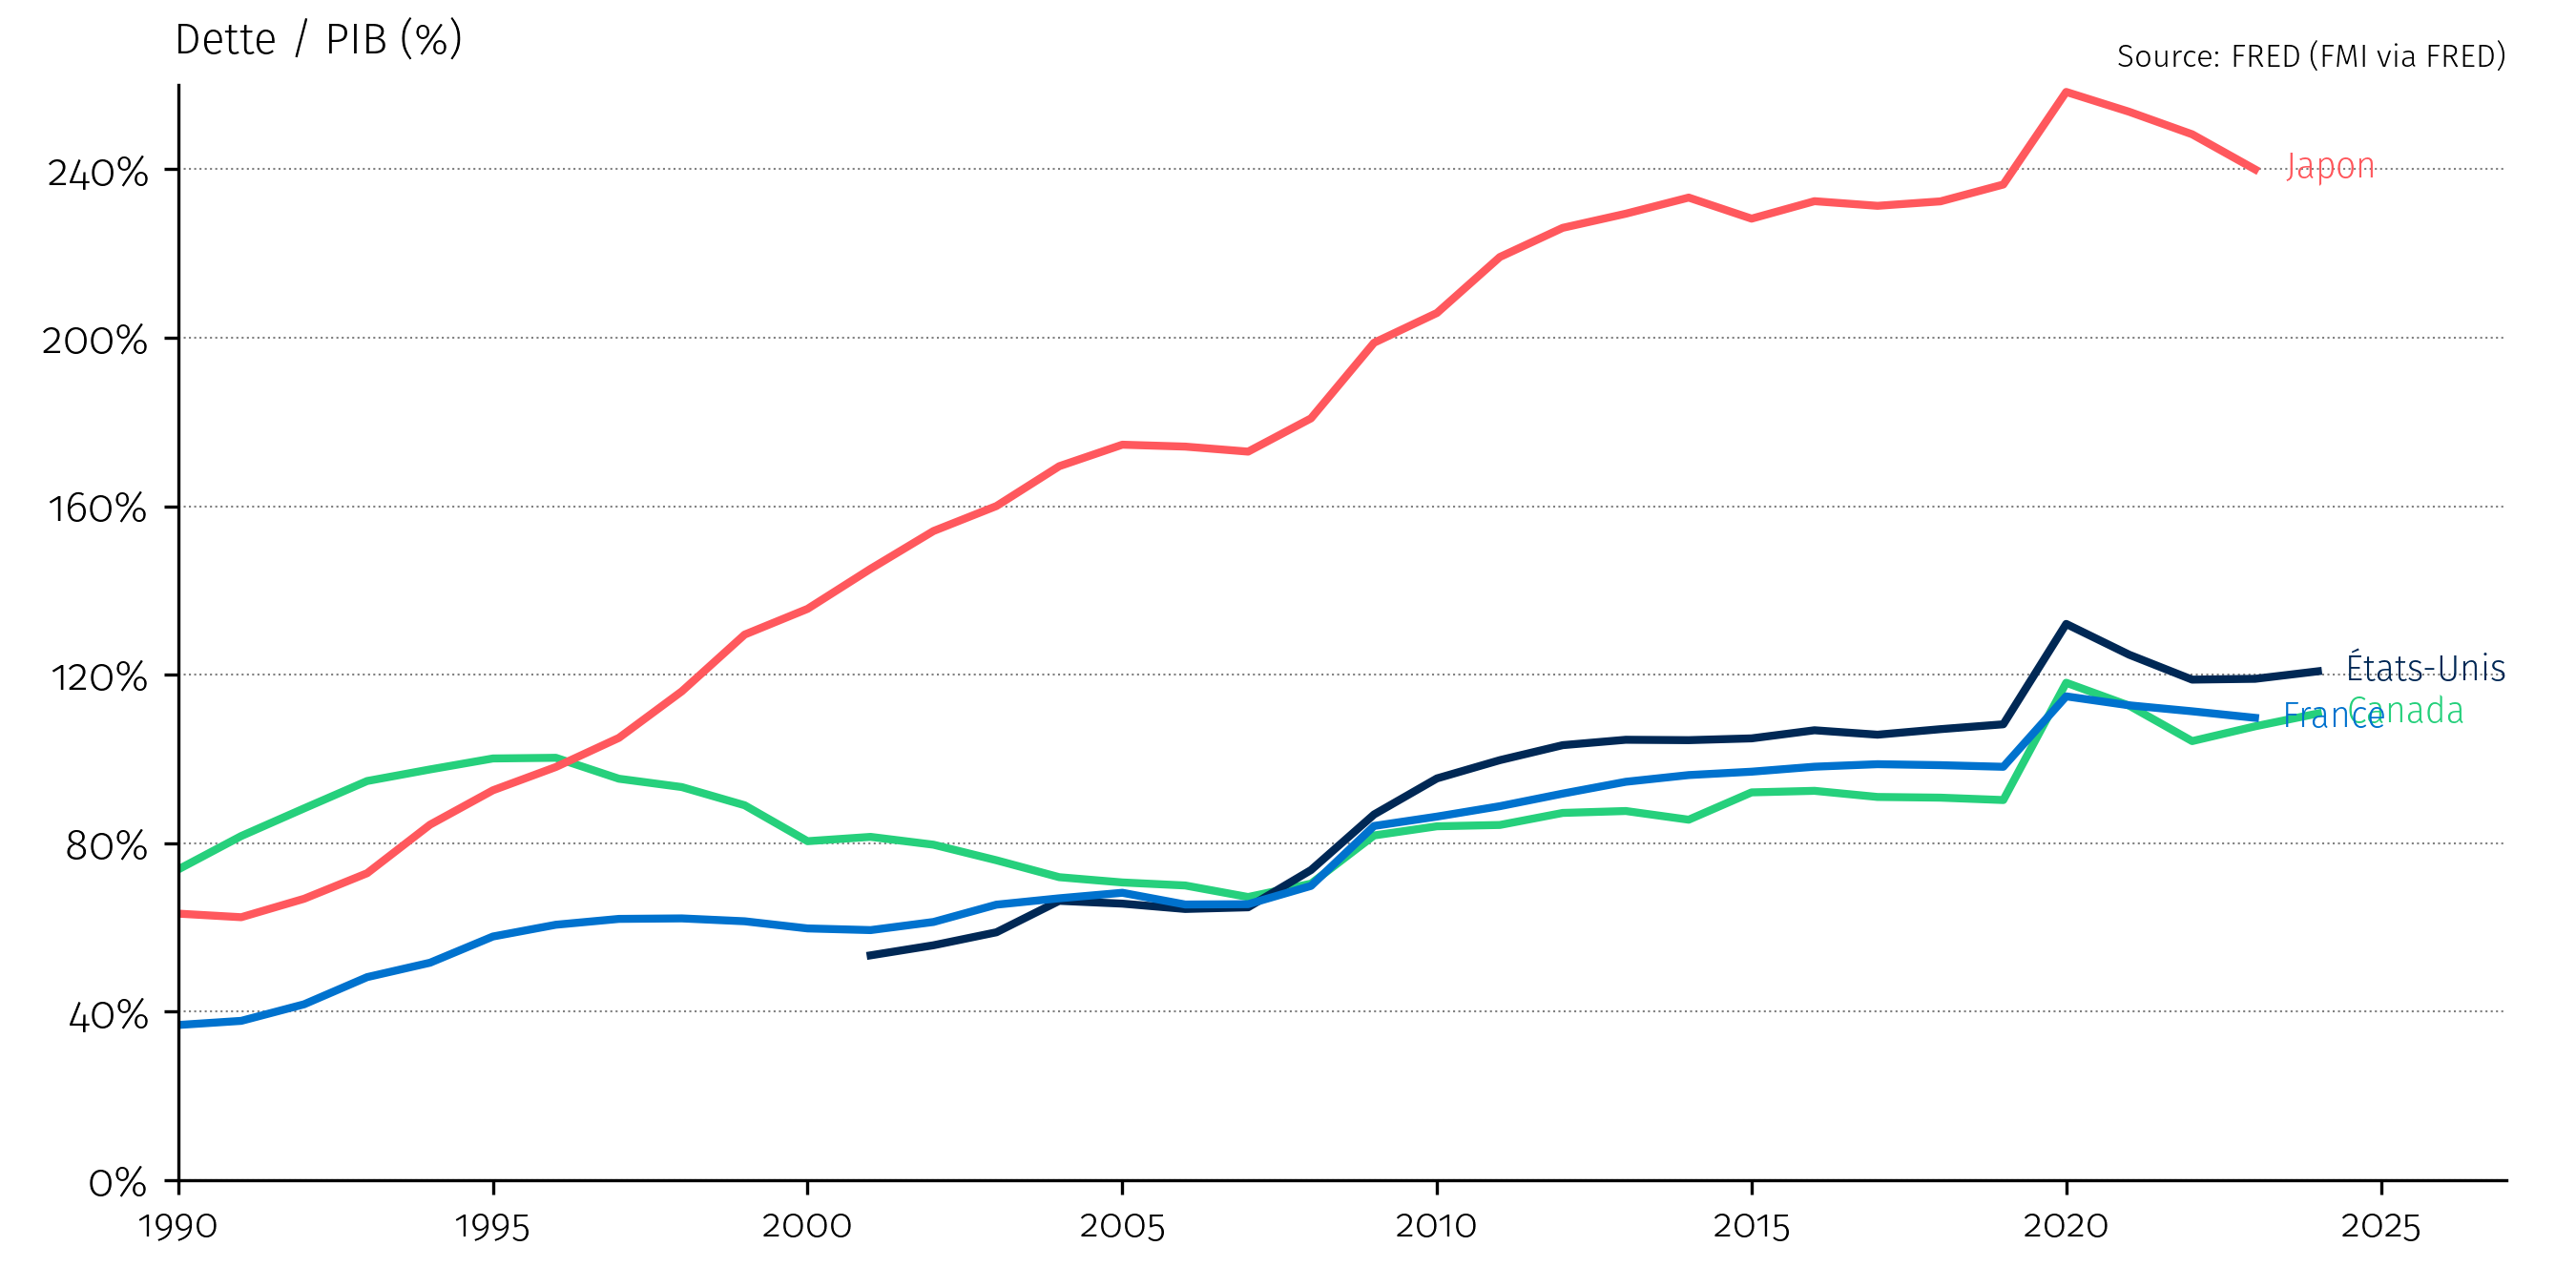
\includegraphics[width=0.95\textwidth, height=0.78\textheight, keepaspectratio]{debt_to_gdp.png}
   \end{figure}
\end{frame}

\begin{frame}[t]{Soutenabilit\'{e} de la dette : la condition $r < g$}
   \small
   \vspace{0.2cm}
   \begin{defbox}[Condition de soutenabilit\'{e}]
      Si le taux d'int\'{e}r\^{e}t sur la dette ($r$) est inf\'{e}rieur au taux de croissance du PIB ($g$), le ratio dette/PIB \textbf{diminue naturellement} --- m\^{e}me sans surplus primaire.
   \end{defbox}
   \vspace{0.15cm}
   \begin{itemize}
      \setlength\itemsep{0.2cm}
      \item \textbf{$r < g$} : la croissance \guillemotleft~dilue~\guillemotright\ la dette $\to$ situation confortable
      \item \textbf{$r > g$} : la dette s'alimente elle-m\^{e}me $\to$ il faut des surplus primaires pour stabiliser le ratio
      \item Depuis 2010, $r < g$ dans la plupart des pays avanc\'{e}s (sauf la crise de la zone euro)
   \end{itemize}
\end{frame}

\begin{frame}[t]{Le pi\`{e}ge de la dette}
   \small
   \vspace{0.2cm}
   \textbf{Quand $r > g$, la spirale s'enclenche :}
   \vspace{0.2cm}
   \begin{enumerate}
      \setlength\itemsep{0.15cm}
      \item Les march\'{e}s doutent de la capacit\'{e} de remboursement
      \item Ils exigent une \textbf{prime de risque} $\to$ $r \uparrow$
      \item La charge d'int\'{e}r\^{e}t augmente $\to$ d\'{e}ficit $\uparrow$ $\to$ dette $\uparrow$
      \item Retour \`{a} l'\'{e}tape 1 (boucle auto-r\'{e}alisatrice)
   \end{enumerate}
   \vspace{0.15cm}
   \textbf{Exemples :}
   \begin{itemize}
      \setlength\itemsep{0.1cm}
      \item \textbf{Gr\`{e}ce (2010)} : dette \`{a} 120\,\% du PIB, taux \`{a} 35\,\% $\to$ d\'{e}faut
      \item \textbf{Italie (2011)} : taux \`{a} 7\,\% $\to$ crise politique, intervention de la BCE
   \end{itemize}
\end{frame}

\begin{frame}[t]{Le Canada est-il en danger\,?}
   \small
   \vspace{0.2cm}
   \begin{columns}[T]
      \begin{column}{0.55\textwidth}
         \textbf{Points rassurants :}
         \begin{itemize}
            \setlength\itemsep{0.15cm}
            \item Dette f\'{e}d\'{e}rale : $\sim$43\,\% du PIB (modeste)
            \item Cote AAA maintenue
            \item Institutions cr\'{e}dibles
            \item March\'{e} obligataire profond et liquide
         \end{itemize}
      \end{column}
      \begin{column}{0.42\textwidth}
         \textbf{Points d'attention :}
         \begin{itemize}
            \setlength\itemsep{0.15cm}
            \item Dette totale (f\'{e}d. + prov.) : $\sim$85\,\%
            \item \textbf{Dette des m\'{e}nages} parmi les plus \'{e}lev\'{e}es au monde
            \item Vuln\'{e}rabilit\'{e} au choc immobilier
         \end{itemize}
      \end{column}
   \end{columns}
   \vspace{0.25cm}
   \begin{warning}
      Le Japon a une dette de 260\,\% du PIB mais emprunte \`{a} des taux tr\`{e}s bas. La Gr\`{e}ce avait 120\,\% et a fait d\'{e}faut. La dette n'est dangereuse que si les \textbf{march\'{e}s doutent}.
   \end{warning}
\end{frame}

\begin{frame}[t]{Dette brute vs.\ dette nette}
   \small
   \vspace{0.1cm}
   \textbf{Dette nette} = dette brute $-$ actifs financiers publics (fonds de pension, r\'{e}serves, placements).
   \vspace{0.15cm}
   \renewcommand{\arraystretch}{1.2}
   \centering
   \begin{tabularx}{0.75\textwidth}{l >{\centering\arraybackslash}X >{\centering\arraybackslash}X}
      \toprule
      \textbf{Pays} & \textbf{Brute (\% PIB)} & \textbf{Nette (\% PIB)} \\
      \midrule
      Japon & $\sim$260 & $\sim$155 \\
      \'{E}tats-Unis & $\sim$125 & $\sim$100 \\
      France & $\sim$112 & $\sim$100 \\
      \rowcolor{HECgreen!12}
      \textbf{Canada} & $\sim$\textbf{105} & $\sim$\textbf{14} \\
      \bottomrule
   \end{tabularx}
   \\[2pt]
   {\footnotesize\textcolor{HECgray}{Source : FMI, \textit{World Economic Outlook} (2024)}}
   \vspace{0.1cm}
   \begin{keyinsight}
      Le Canada poss\`{e}de d'importants actifs publics (RPC, Caisse de d\'{e}p\^{o}t). Sa dette \textbf{nette} est la plus basse du G7 --- une marge de man\oe uvre fiscale consid\'{e}rable.
   \end{keyinsight}
\end{frame}

\begin{frame}[t]{Le vrai risque : la cr\'{e}dibilit\'{e}}
   \small
   \vspace{0.2cm}
   \textbf{Les march\'{e}s fixent le taux, pas le gouvernement.}
   \vspace{0.2cm}
   \begin{itemize}
      \setlength\itemsep{0.2cm}
      \item Si la confiance s'\'{e}rode $\to$ $r \uparrow$ $\to$ spirale de la dette
      \item La cr\'{e}dibilit\'{e} budg\'{e}taire d\'{e}pend de : institutions solides, plan de consolidation cr\'{e}dible, ind\'{e}pendance de la banque centrale
      \item \textbf{Exemple r\'{e}cent :} le Royaume-Uni sous Liz Truss (septembre 2022) --- un mini-budget avec des baisses d'imp\^{o}ts non financ\'{e}es $\to$ livre sterling en chute, taux obligataires en hausse, d\'{e}mission en 45 jours
   \end{itemize}
   \vspace{0.15cm}
   \begin{bizimplication}
      Pour un gestionnaire, la trajectoire de la dette publique est un \textbf{indicateur de risque pays}. Elle affecte les taux d'int\'{e}r\^{e}t, le taux de change et la stabilit\'{e} macro.
   \end{bizimplication}
\end{frame}

% ============================================================================
% CLOSING SEQUENCE
% ============================================================================

\begin{frame}{}
   \centering
   \vspace{1.5cm}
   {\Large\textbf{Qu'est-ce que vous retenez de cette s\'{e}ance\,?}}
\end{frame}

% ============================================================================
\sectionframe{Et pour la suite\,?}
% ============================================================================

\begin{frame}{Th\`{e}mes et s\'{e}ances \`{a} venir}
   \renewcommand{\arraystretch}{1.5}
   \centering
   \small
   \begin{tabularx}{\textwidth}{>{\bfseries}X l}
      \toprule
      \textbf{Th\`{e}me} & \textbf{S\'{e}ance} \\
      \midrule
      Quel avenir pour la mondialisation\,? & S6 : Commerce international \\
      \bottomrule
   \end{tabularx}
\end{frame}

\end{document}
